%\setcounter{secnumdepth}{2}
\chapter{Cardiac Tissue Processing Experimentation}
In the previous chapter, the operation and features of the LSFM, the mesoSPIM microscope, used for acquisition of volumetric images of cardiac tissue were discussed. In addition, it was demonstrated how the mesoSPIM could be utilized as part of the cardiac tissue imaging pipeline through the use of customized mounting, data acquisition, and data processing procedures. This chapter will turn its attention to the cardiac tissue samples themselves and the process by the which they are prepared for imaging utilizing the aforementioned microscopy system and protocols.

\section{Cardiac Tissue Pre-Processing}
Tissue preparation protocols (cardiovascular science protocols in Figure 1.1) discussed in this section were completed by associate researchers in School of Cardiovascular and Metabolic Health at the University of Glasgow College of Medical, Veterinary, and Life Sciences. These associate researchers have the necessary accreditation and training to handle live biological specimens required to obtain tissue samples. All discussed protocols following leporine sacrificing were personally observed and documented (where possible) at least once during the course of research in accordance with existing health and safety guidelines. The declarations at the end of each section will specify which colleagues are credited with conducting which protocols. 

\subsection{Ethics Declaration}

All protocols in this chapter section were approved by the UK Home Office and conforms with the guidance provided in the Animals (Scientific Procedures) Act of 1986. [Freeman, 2023]. The MI induction surgeries were conducted in collaboration with the following staff and researchers of School of Cardiovascular and Metabolic Health at the College of Medical, Veterinary, and Life Sciences at the University of Glasgow: Mike Dunne, Erin Boland, John McAbney, Sasha Forbes, Eline Huethorst, and Mike Freeman.  

In line with the 3Rs (Reduce, Refine, Reuse) of the University of Glasgow's Code of Good Practice in Research, no leporine stock was sacrificed for the exclusive use of this project. All excised hearts were first utilized in projects underway at SCMH (details in Chapter 5) and would have otherwise been examined with standard two dimensional histological methods if not processed for use in this research.


\subsection{Percutaneous MI Model in Leporine Models}
For this project, multiple samples of MI damaged hearts were obtained following the percutaneous leporine MI model developed by the School of Cardiovascular and Metabolic Health (SCMH) at the University of Glasgow [Freeman, 2023]. New Zealand White Rabbits (2.5-3.5 kg) were anaesthetised and underwent a midline incision from the tracheal notch of the rabbit resting in the supine position. The carotid artery is isolated and a small incision is made to allow the insertion of a vascular sheath into the artery. A micro-catheter with radio opaque markers is fed into the sheath into the aorta chamber and through the left coronary ostium via a guide wire. The guide wire is inserted using an angiogram to direct operators inserting the wire where to position the wire. Fluoroscopic projections are used to aid in movement of catheter into the artery with radio opaque markers making the catheter visible in the projections. As the catheter advances into the left coronary artery, a 5 mm micro-catheter tip is deposited in the vessel roughly two-thirds of the distance between the aorta and apex of the heart. The tip will block blood flow through the artery, inducing a moderate infarct in the left ventricle towards the apex.  

\begin{figure}[ht]
    \centering
    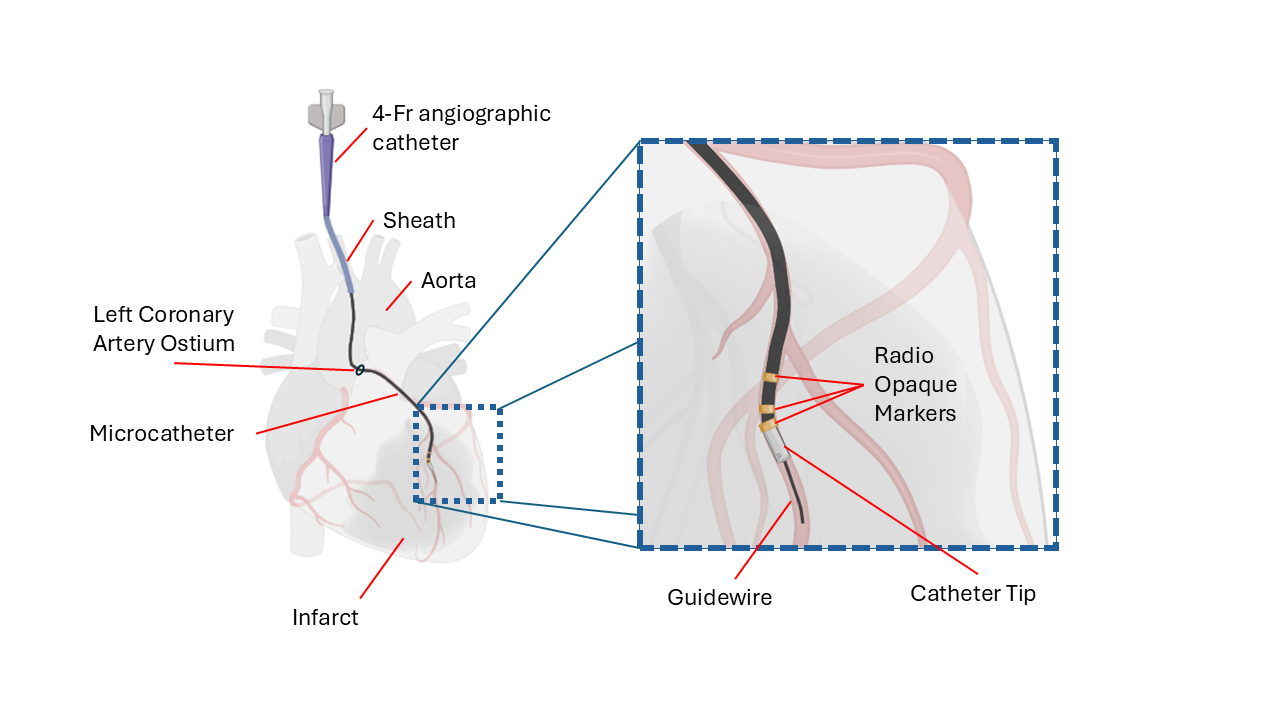
\includegraphics[width=1\linewidth]{Figures/Figure2_2.png}
    \caption{\textbf{Diagram of Rabbit Left Ventricle Percutaneous Occlusion} [Freeman 2023] (Created in  https://BioRender.com)}
    \label{fig:enter-label}
\end{figure}

 Once the infarct is confirmed to have taken place, the guide-wire, catheter, and sheath is removed and the incisions into the artery and the surrounding tissue are sutured closed with the animal receiving post-surgical care. A number of rabbits receive sham operations which leaves the function of the heart unchanged post-surgery. The condition of the treated rabbits is monitored for the next six to eight weeks as the formation of scar tissue and restructuring of the myocardium progresses to completion. Echocardiograms are used to determine the EF of the heart pre and post-MI. 


\subsection{Leporine Heart Isolation}
Once the features of fully developed myocardium restructuring are observed in echocardiogram recordings, the rabbits are euthanised via injection of sodium pentobarbitone and heparin solution to proceed with heart excision. The hearts are then surgically removed from the chest cavity of the rabbit post-mortem prior to the cessation of beating occurs. The still beating heart is then placed into ice-cold Tyrode's solution to stop all remaining cardiac muscle contraction and to prevent the immediate death of remaining healthy cardiac tissue \textit{ex-vivo}. Heart excisions were also performed on healthy animals that underwent sham surgeries (catheter was not used in surgery) to obtain control, healthy rabbit heart samples in addition to MI heart samples.



\subsection{Langendorff Perfusion of Excised Leporine Heart}
Intact rabbit hearts submerged in cold Tyrode's solution are then attached to an Langendorff perfusion assembly by cannulating the aorta on the top of heart directly onto the system using sutures to hold the organ in place. The retrograde perfusion system is then used to pump warm (37 degrees Celsius) Tyrode's solution through the heart chambers and coronary vasculature in the reverse direction blood would normally travel \textit{in vivo}. This perfusion removes any residual blood remaining within the heart. An instance of this perfusion step underway is shown in Figure 2.3.

\begin{figure}[ht]
    \centering
    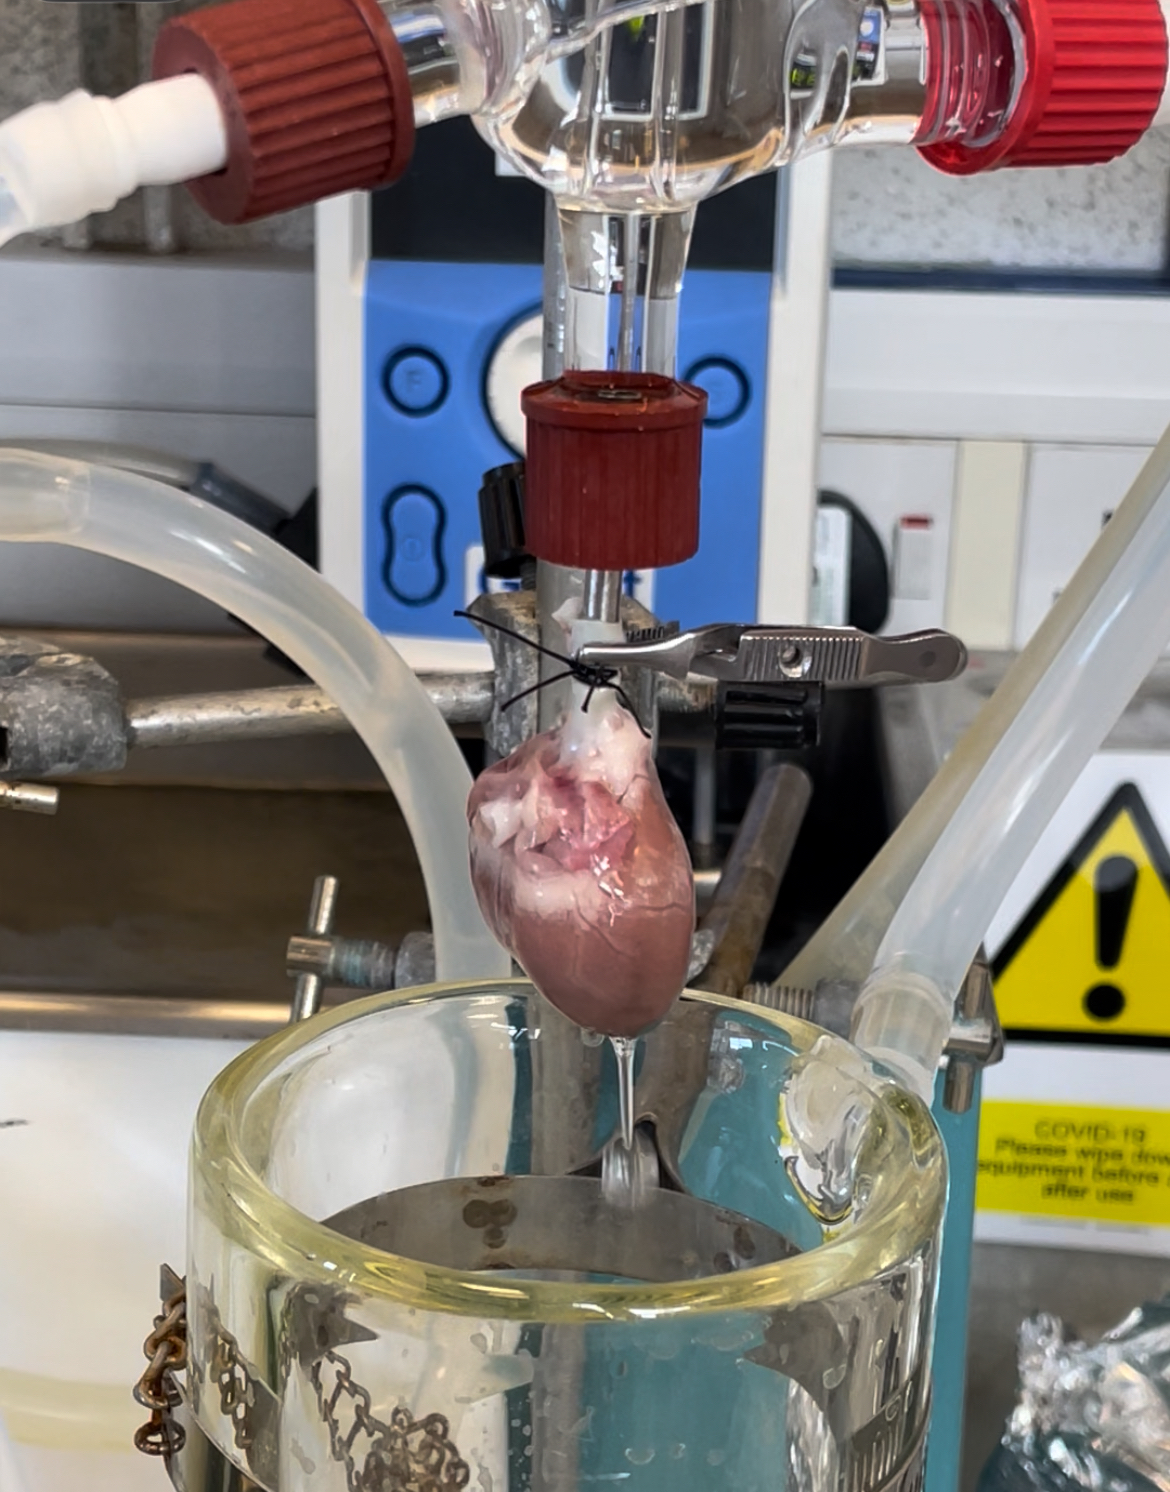
\includegraphics[width=0.5\linewidth]{Figures/Fig2_3.jpeg}
    \caption{\textbf{Intact rabbit heart cannulated onto Langendorff perfusion assembly.}}
    \label{fig:enter-label}
\end{figure}

For samples utilized in this project, all hearts perfused via the Langendorff perfusion were kept alive attached to the system over the course of multiple hours as electrical activity of the organ was recorded with sympathetic activation of the cardiac muscle replicated using attached electrodes. This cardiac tissue functional data was recorded and utilized in a separate research experiment that utilized this imaging pipeline for structural data acquisition that will be discussed in Chapter 5.

Once functional data recordings are complete, the organ is submerged in a 5\% Paraformaldehyde (PFA) solution for fifteen minutes. This is done to fixate the cells in the tissue, permitting long term preservation of tissue structure in-vitro. The LV of the cardiac sample is then excised from the rest of the organ and stored in a solution of 1 mM Phosphate Buffered Saline (PBS) with 0.02 \% Sodium Azide.

\section{Cardiac Tissue Processing Methodology}

The following section will detail the methodologies and experiments conducted to optimize the biochemical steps of the overall imaging pipeline (Steps 3-4 in Figure 2.1). Tissues discussed here will have already undergone all cardiovascular science based pre-processing protocols (detailed in Section 2.1). These protocols were all performed by myself in addition to other members the cardiophotonics research group, in both the School of Physics and Astronomy and the School of Cardiovascular and Metabolic Health at the University of Glasgow, at various point through the course of the project. 

Tissue clearing methods explored in depth during the course of research, CLARITY and CUBIC-L/RA protocols, were already established as effective clearing methods for cardiac tissues in prior publications[]. Clearing methods used here will be based established protocols created by Dr. Camilla Olianti at the University of Siena and the CUBICStars group based at the University of Tokyo with modifications made at several steps. These alterations were implemented to better accommodate the large volumes of 0.4-2.0 mm thick tissues cleared in a given clearing session. Changes were also made to simplify several steps that were found to be particularly laborious or prone to failure.

Due to the long time spans required to complete the tissue clearing process, many of these alterations could only be made after observing the results of prior tissue clearing sessions performed months prior. While further improvements could be made to the protocol, only those most crucial to the optimization of the protocol in the imaging pipeline were implemented.

\subsection{Rabbit Cardiac Tissue Slicing}

Once perfused and fixated, the left ventricle cardiac wall is removed from the remainder of the cardiac tissue using suture scissors. The intact ventricle wall is then cut into 1.0 cm x 2.0 cm wide sections and stored in Phosphate Buffered Saline (PBS) solution. Several of these sections are kept intact for use in hyper-hydrating tissue clearing (see Chapter 3.1.2, CUBIC-L/RA Protocol For Left Ventricle Sections) with the remainder being designated for use in hydrogel-hybridization tissue clearing (see Chapter 3.1.2, CLARITY Protocol) , requiring precision slicing of left ventricle sections.

The left ventricle wall sections are then dried on paper towels before being placed with tweezers into a well plate with a small amount of 20\% agar solution on the bottom of each well. Samples are encased in heated, viscous agar solution, filling the wells of the plate to capacity while forcing out any pockets of air remaining inside. The plate is then stored in cold storage until the agar solidifies (approx. 15-20 minutes). Agar blocks are removed from the well plate and cut into rectangular shapes containing the cardiac tissue section in the centre of the block. 

Cyanoacrylate adhesive is applied to a mounting block and the agar block is placed atop with the epicardium and pericardium of the cardiac tissue oriented perpendicular to the top surface of the block, allowing the adhesive to dry (2 minutes) and secure the block in place. The block with the attached sample is then placed into the specimen bath with the epicardium facing towards the direction of the system’s blade mount. The block is secured using the specimen clamp of a Vibratome Series 1000 Classic Tissue Sectioning System and the specimen bath of the device is filled with PBS solution. A sharpened ceramic blade (Campden Instruments 7550-1-C) is inserted into the Vibratome and locked into position. The device is then activated and set to the highest position and slowest speed setting to begin slicing the top of the agar block in increments of 2.0 mm until the blade reaches the top of the cardiac tissue embedded inside.

As the ceramic blade begins cutting through cardiac tissue, the device is paused and the system is set to begin cutting the tissue in intervals of 0.4 mm, 0.5 mm, 1.0 mm, and 2.0 mm. Each slice is recovered from the specimen bath using pipette tips as they separate from the block. Agar remaining around the slice is carefully removed and the remainder of the tissue slices are stored in labelled containers containing PBS. The protocol is repeated for each agar block created until all tissue is sliced and stored. Vibratome operation is monitored throughout to ensure the blade does not pull out the cardiac tissue from the agar or the agar block is pulled from the mounting block beneath it. Suture scissors are used to cut any fibrous strands still connecting a slice to the agar block should they not be severed by the ceramic blade. 
The slice taken from top of the embedded slice, along with any partial slice or tissue fragments that broke off during the slicing process, are disposed into biohazard waste. Once slicing is complete, the ceramic blade is carefully removed and cleaned. The system mounting block is cleaned of residue with the remainder of the Vibratome specimen bath and blade holder cleaned using ethanol solution and deionized water


\subsection{Cardiac Tissue Clearing}
\subsubsection{Pre-Clearing Tissue Expansion Documentation}

To determine the expansion rate of tissues that undergo clearing protocols,  images of each tissue slices was taken by myself with a 12 Megapixel Apple iPhone 12 Pro camera. Left ventricle sections were captured using a 10 Megapixel Samsung Galaxy s23 FE camera by Dr. Eline Huethorst. Each tissue slice is removed from post-slicing PBS storage container and laid flat into 50 mm diameter petri dish.  Beneath the transparent dish was laid graph paper with millimetre grid squares. Sliced tissues were rotated to have (as best a possible) the epicardium edge of the tissue to be parallel to the lines of the grid paper beneath. LV sections are laid with one transmural face flat on the dish, the other face facing the camera, the epicardium side on the right, and endocardium on the left. Once positioned, labels are placed in the field of view of the camera containing details on the sample (identifier, thickness, tissue condition) and the image is captured. Process is repeated for each tissue just prior to start of clearing protocols. 

\subsubsection{\textit{CLARITY Protocol}}

The clearing protocols performed and modified for use in this research is based on the tissue clearing protocols developed by Dr. Camilla Olianti []. A diagram of the overall process is shown in Figure 3.1 below:

\begin{figure}[H]
    \centering
    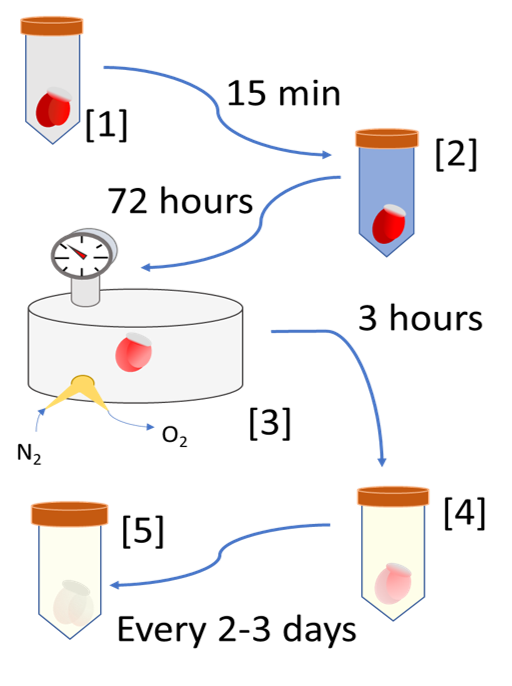
\includegraphics[width=0.5\linewidth]{Figures/Figure3.1.png}
    \caption{\textbf{CLARITY protocol process diagram.} Steps: [1] Tissue slices washed in PBS for 15 min, [2] Tissue washed in hydrogel solution for 72 hours, [3] Tissue degassed in nitrogen ($N_2$) gas for 3 hours, [4] Tissue washed in detergent solution, [5] Detergent solution changed out every 2-3 days for 5-7 months.}
    \label{fig:enter-label}
\end{figure}

For the clearing of sliced cardiac tissues using CLARITY clearing protocol, Hydrogel and clearing stock solutions were made. Hydrogel stock solution: 875 ml deionized water, 2.5 g Initiator AF-067, 100 mL Acrylamide, and 25 mL Bis-Acrylamide was mixed using magnetic stirring plate under a fume hood. Once sufficiently stirred, the solution is stored in sealed containers at -20 degrees Celsius for up to 12 months. The frozen stock is left to thaw for 12 hours prior to future use in the protocol. 
For CLARITY clearing stock solution: 5 L deionized water, 61.833 g Boric Acid, 220 g Sodium Doedecylsulfate (SDS) were mixed with a magnetic stirrer under fume hood. Sodium Hydroxide was added one drop at a time until a pH meter inserted into solution while it stirred recorded a stable a pH of 8.5. Clearing solution was then stored at room temperature inside a sealed 25 L container. Solution is occasionally re-stirred to prevent build-up of solute deposits over several months.

Sliced tissue samples stored in PBS are prepared for hydrogel solution immersion by being drained of PBS solution and being laid carefully atop microscope slides ensuring no folds or twisting of the tissue slice is present. A second microscope slide is laid atop the tissue slice ensuring no bubbles emerge between the slides and surface of the tissue. Once bubbles have been removed, the sandwiched sample is inserted into a 3D printed mount holder containing an internal spacer of equal thickness to the sample between the slides (see Chapter 4.1 for details on mount design). The mount is then sealed with a two-part curing silicone, ensuring a watertight seal on both sides of the mounted sample. 

After leaving silicone to dry for 15 minutes mounts are placed into sealable glass containers and injected with thawed hydrogel solution. Mounts are injected using 0.45 mm diameter injection needles attached to 1.0 ml syringe. During injection, mounts are inspected to ensure no bubbles form inside the mounts near the tissue slices. Once filled, the remaining volume of the glass containers is filled with hydrogel solution before being sealed closed and stored at 4 degrees Celsius with stirring for 72 hours. 
After 72 hours, samples are removed from the fridge and placed into a vacuum chamber under a fume hood with the lids of each glass container unsealed and left loose atop each container. A vacuum pump is then used to remove air from the chamber. Once a reading of -0.8 MPa is recorded, the pump is stopped, and the chamber is filled with nitrogen gas, $N_2$. Once the chamber returns to atmospheric pressure, the lid of chamber is opened, and each container lid is quickly closed to entrap Nitrogen gas inside. Nitrogen flooded containers are thereafter stored without stirring at 37 degrees Celsius for 3 hours. 

Upon completion of incubation, each sample is carefully removed from the sealed containers and custom 3D printed mounts. Excess hydrogel around the tissue slices is removed and the samples are gently deposited into labelled well plates containing 15 mL of 8.5 pH balanced CLARITY clearing solution in each well. Lids are place over each well plate and samples are stored inside at 37 degrees Celsius with stirring for 5 to 10 months while lipids gradually diffuse out of the tissue slices. Clearing solution inside each well is removed and replaced with fresh stock solution three times a week for the duration of this clearing period with monthly inspection of samples undertaken to monitor progress of lipid diffusion in each sample. As individual samples reach completion of lipid diffusion (starting at 5 months for thinner sliced tissues), the sample is removed from the well plates and washed three times in 1x PBS for 1 hour to prevent SDS precipitation. After washing, the samples are stored at 4 degrees Celsius in a solution of 10 mM PBS/ 4\% Sodium Azide ($NaN_3$) for up to 3 months. 


\subsubsection{\textit{CUBIC-L/RA Protocol for Left Ventricle Sections}}

The clearing protocols performed and modified for use in this research is based on the tissue clearing protocols developed by CUBICStars []. A diagram showcasing the steps in this procedure is shown in the following Figure:

\begin{figure}[H]
    \centering
    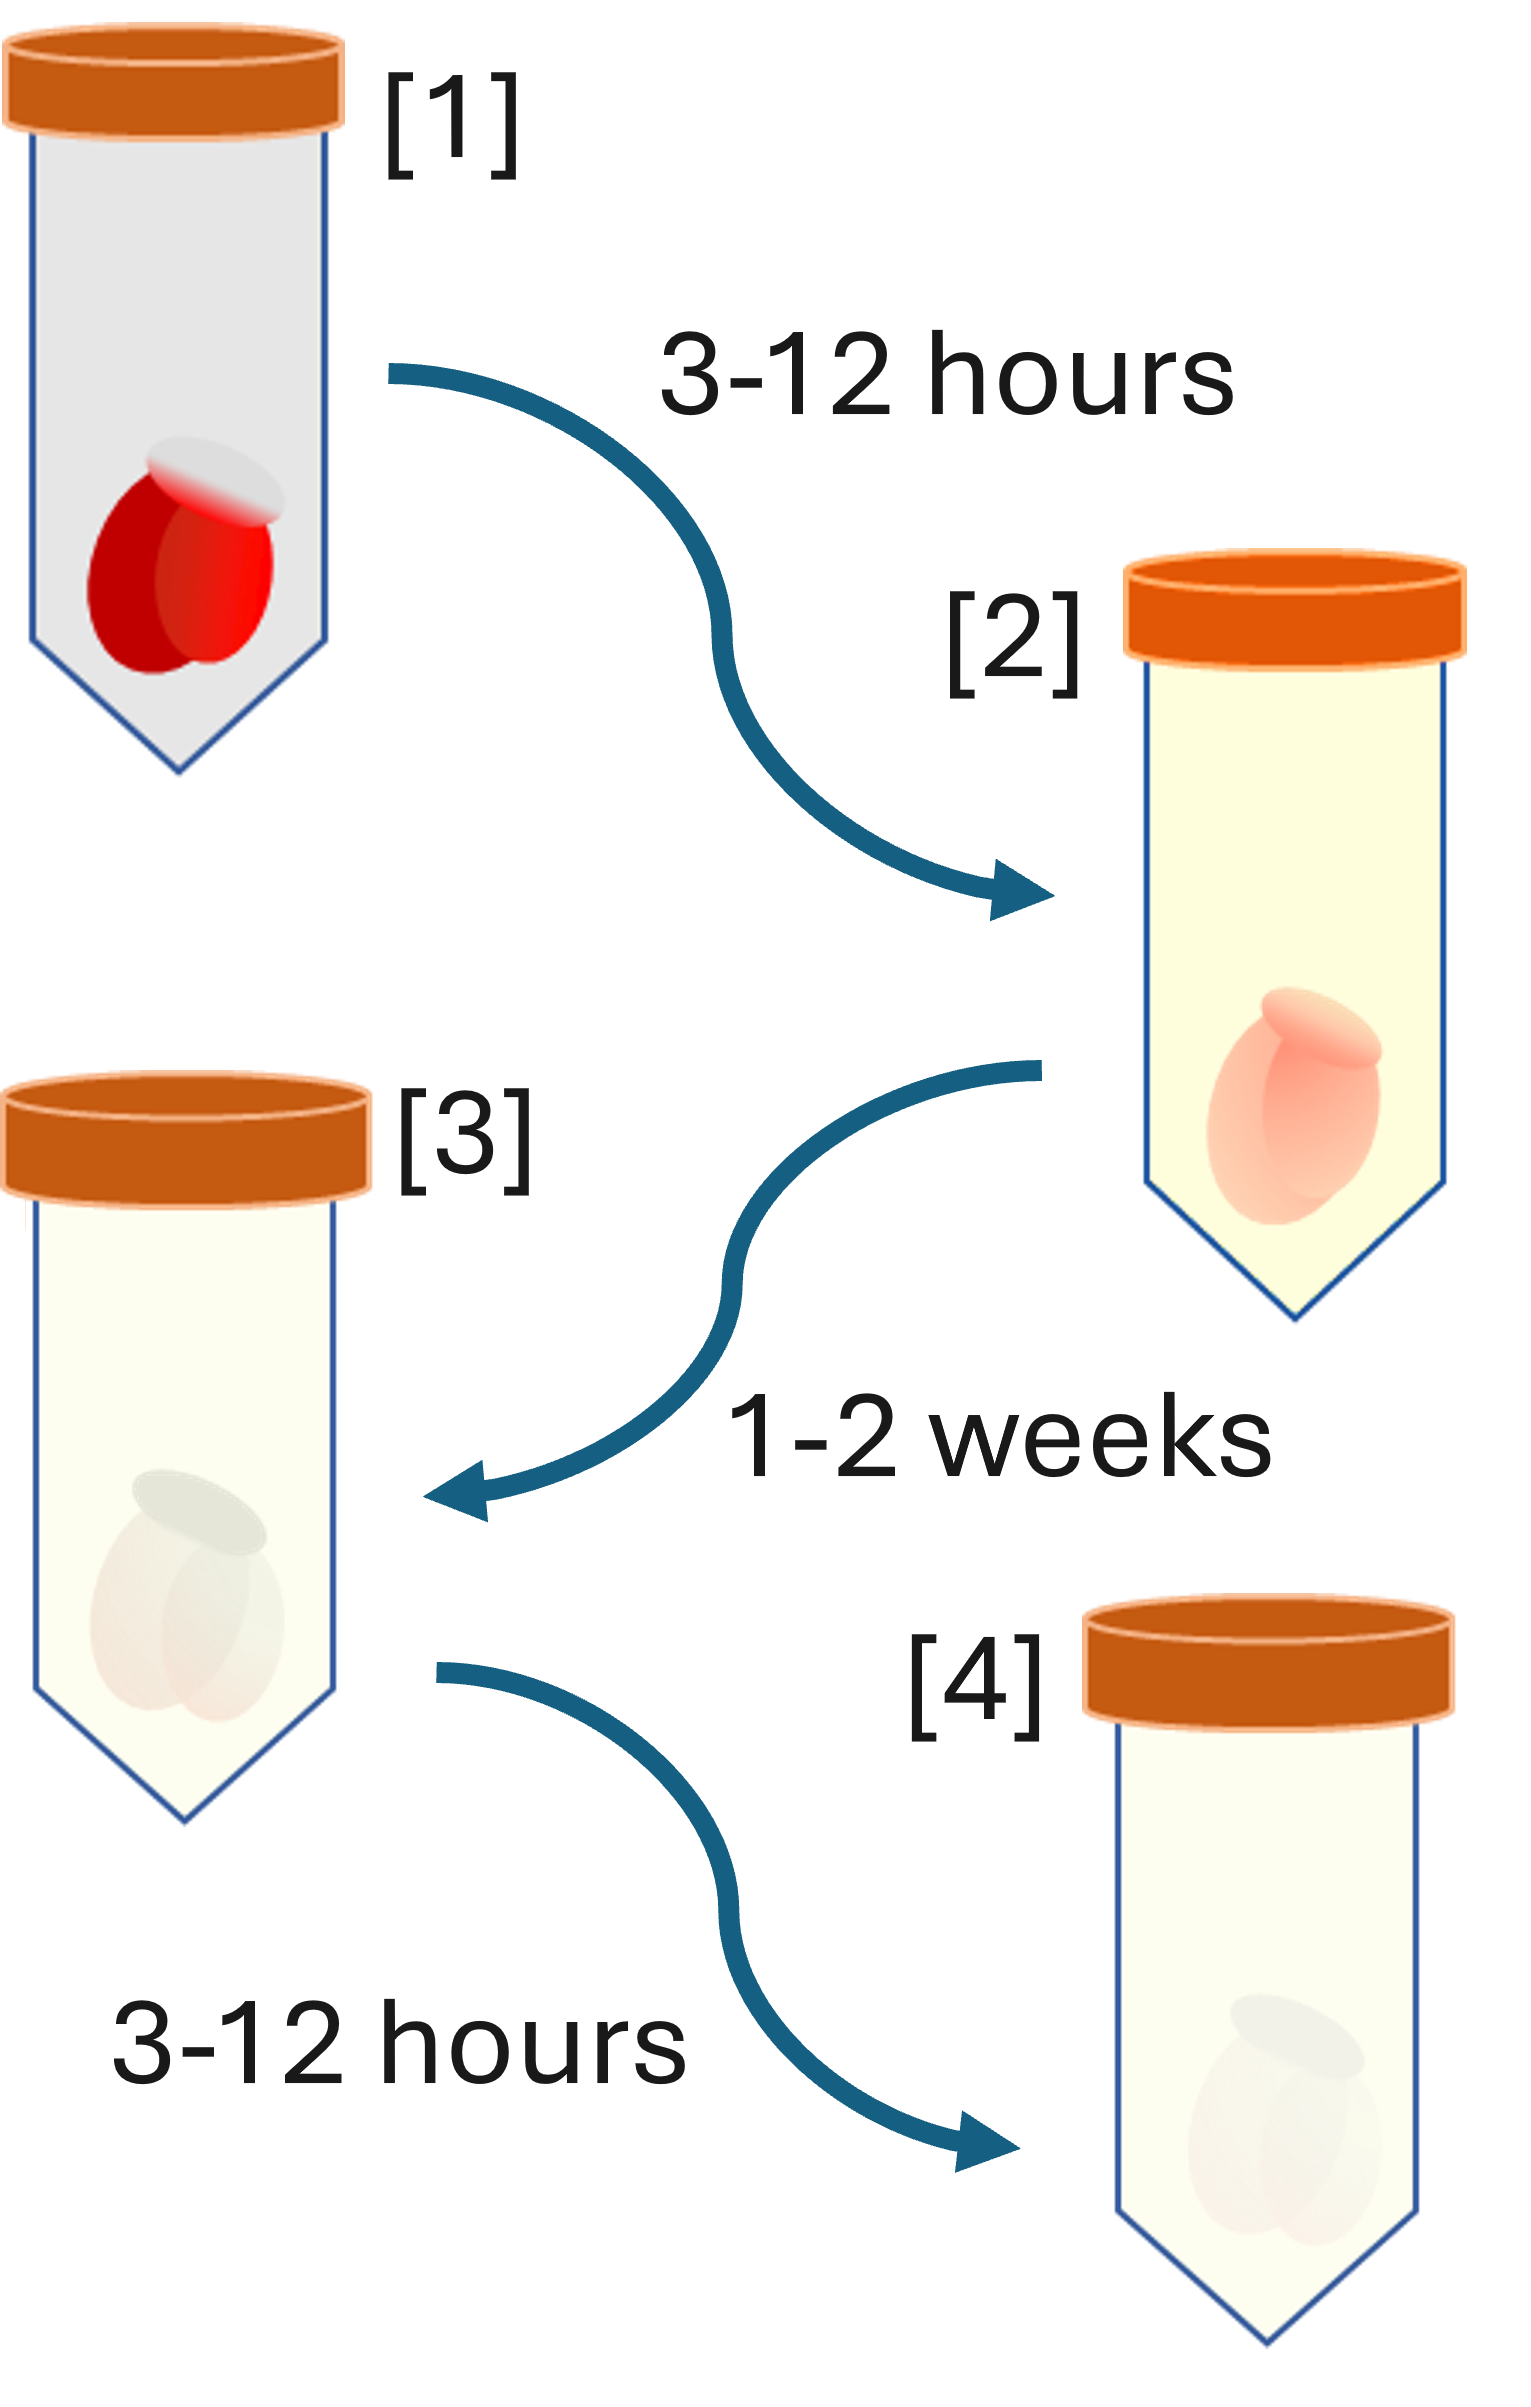
\includegraphics[width=0.5\linewidth]{Figures/Figure3.2.png}
    \caption{\textbf{CUBIC-L/RA protocol process diagram.} Steps: [1] Tissue washed in 50\% CUBIC-L solution for 3-12 hours, [2] Tissue washed in CUBIC-L for 7 to 14 days, [3] Tissue washed in 50\% CUBIC-RA Solution for 3-12 hours, [4] Tissue Washed in 100\% CUBIC-RA for 2-3 weeks.}
    \label{fig:enter-label}
\end{figure}


For 100 mL CUBIC-L stock solution: 10 mL N-Butyldiethanol is dissolved in 60 mL deionized water using a magnetic stirrer under fume hood. Once fully dissolved, 10 mL Triton X-100 and and additional 20 mL of deionized water are added and left to mix thoroughly for several minutes. Solution is stored under the fume hood in a sealed container, occasionally re-stirred to prevent any build-up of solute deposits.

Left ventricle tissue samples stored in PBS are drained and inserted gently into a 50 mL test tube filled with 50\% CUBIC-L Solution in deionized water and washed for 12 to 24 hours with gentle agitation. Once done, samples are placed in a test tube with 100\% CUBIC-L stock solution. The tube is sealed closed and stored at 37 degrees Celsius for 1-3 weeks until fully saturated with the solution, rendering the complete volume of the tissue translucent when held up to a light-source. CUBIC-L solution is changed out every 2-3 days for the duration of this clearing period. Samples in CUBIC-L solution may be kept for slightly longer past the three week if required to achieve full translucence across the entire sample volume, but for no more than four weeks to prevent tissue degradation from prolonged protein denaturing. After this, CUBIC-L cleared samples are removed from sealed containers and washed three times in 1x PBS for 1 hour to prevent CUBIC-L solute precipitation. After washing, the samples are stored at 4 degrees Celsius in a solution of 1x PBS/ 4\% Sodium Azide (\(NaN_3\)) for up to 3 months.

Immediately prior to immersion in CUBIC-RA, CUBIC-L treated samples can be stained with a florescent dyes of choice. Which and how many dyes are used will vary depending on the aspects/types of structures in the sample a user is attempting to identify and record using this pipeline.  Staining protocols times will vary, but all will concluded with sample being fixated immediately after in PBS/ 4\% PFA solution followed by a triple wash in stock 1x PBS. Dye florescence is preserved by keeping samples away from all light sources for the remainder of this pipeline. 

Once tissues have undergone staining and washing procedures, samples are immersed in an aqueous 50\% solution of CUBIC-RA (Tokyo Chemical Industries T3741) mixed thoroughly with deionized water for 12 to 24 hours. The sample is removed from this solution and positioned inside an optical glass cuvette (Portmann Instruments UG-205) using pipette tips to gently orient the sample so the epicardium is flush against the internal wall of the cuvette. Should the sample be found to be thinner than the internal width of the cuvette (10 mm), a bed of 5\% agarose (20 mm x 40 mm) is placed behind the sample to fill the remaining space and keep the sample fixed in place in the front half of the cuvette volume. Agarose beds of varying thicknesses (2 mm, 3 mm, and 5 mm) are made beforehand to allow the best fitting bed to be used if and when needed. The internal cuvette is then filled with 4-5 mL of 100\% CUBIC-RA stock solution. Pipette tips are used to remove any bubbles or air pockets that form after cuvette is filled. CUBIC-RA will thereafter RI match left ventricle samples to the solution and optical glass cuvette over the course of 5-7 days. Thicker slices (1-2mm) can require additional time immersed to achieve greatest degree of RI matching possible. The cuvette is covered and kept away from light sources for duration of RI matching period to preserve tissue florescence (if any). 

\subsection{Post-Clearing Tissue Processing}
\subsubsection{\textit{Cleared Tissue Long Term Storage}}

Tissues cleared using CLARITY monitored through the final step of the protocol, washing in from the incubator as they form over the course of several weeks. Clearing solution was changed out three times a week to prevent the clearing process from decelerating due to a saturation of extracted lipids in the solution over time or by the gradual evaporation of solution in the heated environment. 
Completion of clearing was determined by the elimination of yellow and light brown coloured hues from any region of the tissue as clearing progressed. Once the tissue was completely transparent with the only remaining colouration in the tissue volume, if any, is pale white. Once a tissue reaches this point, it signifies a sufficient removal of pigmentation and lipids with negligible amounts remaining. The slices are then placed into sealable containers containing a solution of 1x PBS with 0.1\% (\(NaN_3\)). These containers are labelled, sealed, and placed in cold storage for preservation of the samples for up to three months.   
Crystallization of residual Sodium Dodecyl sulphate was found on occasion to form on the surfaces of the tissue shortly after placement in long term fridge storage. This was most often seen on thicker tissue slices greater than 1mm in thickness and formed because of detergent inside the tissue gradually diffusing into the cold 1x PBS/\(NaN_3\) solution where it began to crystallize. To prevent the crystallization from damaging the tissue, any samples found to have excessive crystallization were placed back into the incubator to allow the detergent to dissolve back into the solution. Once dissolved, the detergent saturated solution was extracted, and fresh \(PBS/NaN_3\) stock solution was added to the sample before returning to cold storage. This tissue would thereafter be monitored for further crystal formation after a week in the new solution. Should any occur, this procedure would be repeated until excessive crystallization ceases in each sample after a week in storage.

\subsubsection{\textit{Tissue Expansion Documentation}}

To determine the expansion rate of tissues that underwent clearing protocols, images of each tissue slice are taken prior to fluorescent staining protocols with a 10 Megapixel digital camera(CANON, PowerShot A640) attached to a dissection microscope (Zeiss, Stemi 2000-C). This system is required with cleared tissues to better discern now faint tissue edges and to reduce artefacts caused by shadows and movement seen when using smartphone cameras. 

Each tissue is removed from post-clearing long term PBS/Sodium Azide storage and laid flat into a 50 mm diameter petri dish beneath the objective of the dissection microscope. A pipette is used to drain any remaining PBS solution around the edges of the tissue. Care is taken during draining to not damage the tissue surface of edges in the process. 
Beneath this transparent dish was placed graph paper with \(1mm^2\) grid squares. The petri dish containing the tissue was rotated to have the tissue match as best as possible the orientation of the tissue seen in pre-clearing image recorded for the sample. Once correctly oriented, the tissue identifier is written in the field of view of the camera and the multiple photos are captured of the tissue at a variety of lighting and zoom settings to best define the edges of the cleared tissue. Once taken, the captured photos are examined to determine if any images are low resolution or poorly illuminated. Camera settings are adjust as needed and images are retaken until high resolution; homogeneous lighting conditions are recorded. All images are recorded onto a SD card as JPG files for image analysis.

\subsubsection{\textit{Tissue Washing and Staining}}
Tissue washing and staining protocols vary depending on the structural features of the cardiac samples being examined in a given research project. As such, there is no one specific protocol to be followed for cleared tissues processed through the imaging pipeline to this point as the samples are intended to be viable for any number of staining techniques currently utilized for biological analysis.

For the purposes of this research, two staining methods (Wheat Germ Agglutin (WGA) Conjugate with Immunohistochemisty (IHC), WGA Conjugate with Nucleic Acid Stain) were performed to demonstrate the versatility in staining these cleared samples posses. These staining combinations were implemented as part of the application of this pipeline into two separate experimental investigations being conducted in collaboration with researches in the School of Cardiovascular and Metabolic Health. Details regarding the customized tissue washing and staining protocols unique to each of these research projects are discussed alongside full application context and detailed results in Chapter 5.


\section{Analysis of Tissue Processing}
\subsection{Analysis of Tissue Clearing}
Successful implementation of the tissue clearing techniques require that the samples respond to the process in a consistent and predictable manner for biological analysis of the cleared tissue to be considered reliable for use in ex vivo study. Extensive prior research exists which examines the effects CLARITY and CUBIC-L/RA clearing methods have on cardiomyocytes []. While this information provides a comparison by which clearing in this research can be compared, the unique combination of mesoscale tissue slicing, mounting as well as the use of rabbit animal model makes direct quantitative comparisons to these prior results unreliable in determining the quality of the clearing obtained in the imaging pipeline.

With that, a quantitative analysis of the impact tissue clearing has on the dimensions, transparency, and structural integrity of the cardiomyocyte samples was performed to rectify the matter. This analysis will provide data that can be used in direct comparison by future practitioners of the imaging pipeline to confirm the successful implementation of the tissue clearing methods in pipeline samples and the reliability of the biological data they contain. 

\subsection{Tissue Expansion After Clearing Protocol}
Changes to the dimensions of the tissue samples post-clearing are anticipated as they have been well documented in past publications []. These changes are an indirect result of the biochemical reactions that occur within the tissue that renders the volume optically transparent. Any dimension expansion that occurs must be quantified so the dimensional change can be taken into consideration when measuring the distances between structure and regions of interest observed within the sample volume. As the tissue expands homogeneously, the equation used to calculate CE of tissue Surface Area is simplified to:

\newline
\begin{equation}
Coefficent\ of\ Expansion\ (CE)= \frac{Surface\ Area_{Post\ Clearing}}{Surface\ Area_{Pre\ Clearing}} 
\end{equation}
\medskip

To determine if the average CE value calculated provides a reasonable estimate of expansion to use in calculations across all tissues in a given category of cleared samples (scarred, healthy, overall), the Coefficient of Variation is calculated following this established equation:

\newline
\begin{equation}
Coefficent\ of\ Variation\ (CV) = \frac{Standard\ Deviation}{Average}*100\%\ [REF]
\end{equation}
\medskip

A low CV value $(\leq 10\%)$ will indicate that the range of CE values calculated are across a small enough range if values for the average to be used as a precise estimate across all samples []. Should the CV be calculated to be high $(\geq 25\%)$, it would suggest the average is a poorer estimate due to the larger range of values of CE values recorded [].

\subsubsection{\textit{CLARITY Expansion}} Tissue expansion in past research was seen to be far more heterogeneously in the axial plane than in the lateral. As such, this heterogeneous expansion in the vertical plane was prevented through the use of a mount in the clearing protocol (as described in Chapter 3), lateral expansion is the sole variable that must be determined for use in proper biological analysis. This variable, defined as the Coefficient of Expansion (CE), will be determined for the lateral surface area of cleared, sliced tissues. Surface area expansion measurements will provide the coefficient required for future biological analysis of the cleared sample including the measurement of tissue structures such as blood vessels and the calculation of cardiomyocyte density in observed tissue regions including scarred, healthy, and border zones in samples with scars.

\subsubsection{\textit{CUBIC-L/RA Expansion}} Slight tissue contraction (CE < 1.0) had previously been observed after immersion in the CUBIC-L substrate but was far less significant in scale compared to CLARITY []. Cardiac tissue samples in particular are found to return to their original, pre-clearing volume and dimensions[]. It is essential to confirm this remains the case when CUBIC-L/RA clearing technique is implemented as part of the tissue imaging pipeline established. This will be done by using both leporine left ventricle tissue slice and sections for expansion analysis. 

The CE for a healthy, sliced tissue cleared with CUBIC-L/RA will be follow the same methodology used for determining Surface Area CE for CLARITY samples. This sample will be used as a direct comparison to the lateral expansion seen in a healthy CLARITY sample of equal thickness. 

For expansion in Left Ventricle Sections cleared using CUBIC-L/RA, axial expansion measurement will be performed on LV sections cleared using CUBIC-L/RA. As expansion in CUBIC-L/RA is found to occur homogenously in the axial plane, the change seen for the width of the LV section (distance from transmural cut to transmural cut) should be negligible upon completion of clearing process. Pre-clearing photos were placed side by side with post-clearing photos to ensure identical locations along the width of each sample were measured roughly midway along the length of each section.

\subsubsection{\textit{Methodology}}

Using Fiji ImageJ software, pre-clearing and post-clearing images of the tissue are measured to calculate the tissue surface area m. Step by step ImageJ protocols for surface area expansion analysis is shown in Figures 3.1. 

\begin{figure}[H]
      
    \begin{subfigure}[t]{.475\textwidth}
    \centering
    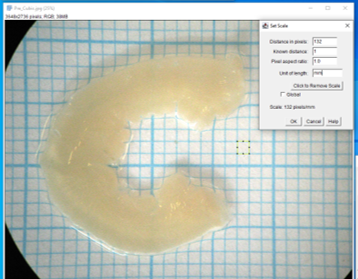
\includegraphics[width=\linewidth]{Figures/MeasureProt1.png}
    \caption{Image scale set using millimetre grid}
    \end{subfigure}\hfill
    ~
    \begin{subfigure}[t]{.475\textwidth}
    \centering
    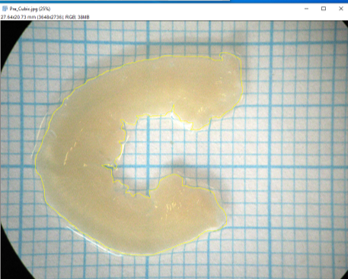
\includegraphics[width=\linewidth]{Figures/MeasureProt2.png}
    \caption{Custom ROI drawn following the edges of the tissue around surface perimeter}
    \end{subfigure}\hfill
    
    \medskip
    \begin{subfigure}[t]{.475\textwidth}
    \centering
    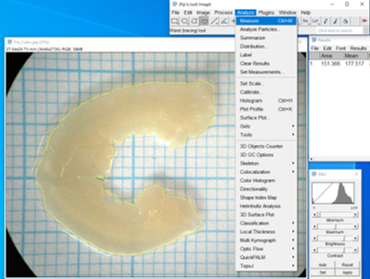
\includegraphics[width=\linewidth]{Figures/MeasureProt4.png}
    \caption{ROI Surface Area measured using Measurement Feature}
    \end{subfigure}\hfill
    ~
    \begin{subfigure}[t]{.475\textwidth}
    \centering
    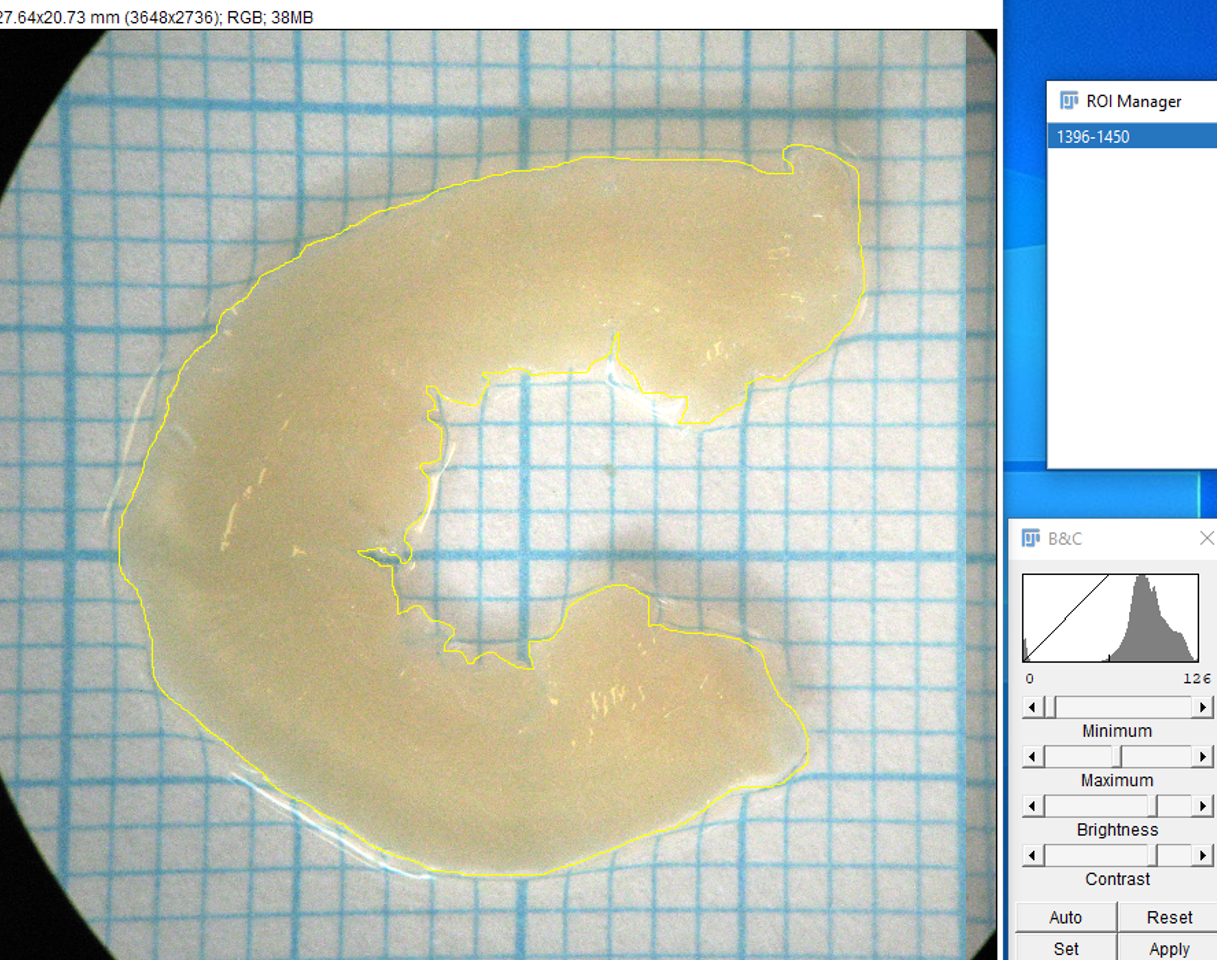
\includegraphics[width=\linewidth]{Figures/MeasureProt3.png}
    \caption{ROI recorded using ImageJ ROI Manager}
    \end{subfigure}\hfill

     \medskip
    \begin{subfigure}[t]{.475\textwidth}
    \centering
    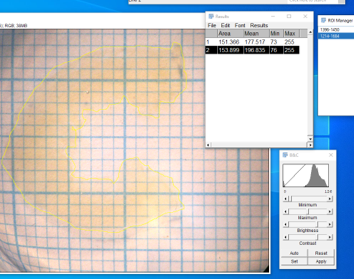
\includegraphics[width=\linewidth]{Figures/MeasureProt5.png}
    \caption{Steps a-d repeated for post clearing image of tissue}
    \end{subfigure}\hfill
    ~
    \begin{subfigure}[t]{.475\textwidth}
    \centering
    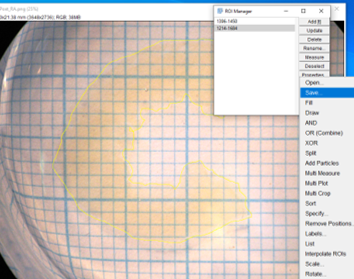
\includegraphics[width=\linewidth]{Figures/MeasureProt6.png}
    \caption{Custom Pre/Post ROIs saved in ZIP file}
    \end{subfigure}\hfill
    
    \caption{\textbf{Surface area expansion coefficient ImageJ measurement protocol}}
    \label{fig:enter-label}
\end{figure}


\subsubsection{\textit{CLARITY Results}}

Expansion coefficient of the tissue surface area was determined for every sample that underwent CLARITY clearing, fluorescent staining during experimentation. Average SA Tissue Expansion Coefficient for scarred and healthy tissue sample sets were then calculated along with standard deviations and standard errors observed in each sample population. These results were plotted in the following figure:  
 

\begin{figure}[H]
    \centering
    \begin{tikzpicture}
        \begin{axis}
        [
        scale = 1,
        ytick={1,2,3},
        yticklabels={Overall,Healthy, Scar},
        boxplot/box extend=0.25
        ]

\addplot+ [
        boxplot prepared={draw position=1,
          median=1.97,
          upper quartile=2.72,
          lower quartile=1.71,
          upper whisker=3.42,
          lower whisker=1.43},
        ] table [y index=0] {Data/Figure3.3.dat}
        [above]
        node at
          (boxplot whisker cs:\boxplotvalue{lower whisker},1)
          {\pgfmathprintnumber{\boxplotvalue{lower whisker}}}
        node at
          (boxplot box cs: \boxplotvalue{median},1)
          {\pgfmathprintnumber{\boxplotvalue{median}}}
        node at
          (boxplot whisker cs:\boxplotvalue{upper whisker},1)
          {\pgfmathprintnumber{\boxplotvalue{upper whisker}}}
        ;
        
\addplot+[
        boxplot prepared={ draw position=2,
          median=1.98,
          upper quartile=2.03,
          lower quartile=1.67,
          upper whisker=2.03,
          lower whisker=1.67},
        ] table [y index=1] {Data/Figure3.3.dat}
        [above]
        node at
          (boxplot whisker cs:\boxplotvalue{lower whisker},1.2)
          {\pgfmathprintnumber{\boxplotvalue{lower whisker}}}
        node at
          (boxplot box cs: \boxplotvalue{median},-2)
          {\pgfmathprintnumber{\boxplotvalue{median}}}
        node at
          (boxplot whisker cs:\boxplotvalue{upper whisker},1.2)
          {\pgfmathprintnumber{\boxplotvalue{upper whisker}}}
        ;
\addplot+[
        boxplot prepared={draw position=3,
          median=1.96,
          upper quartile=3.18,
          lower quartile=1.62,
          upper whisker=3.42,
          lower whisker=1.43}
        ] table [y index=2] {Data/Figure3.3.dat}
        [above]
        node at
          (boxplot whisker cs:\boxplotvalue{lower whisker},1)
          {\pgfmathprintnumber{\boxplotvalue{lower whisker}}}
        node at
          (boxplot box cs: \boxplotvalue{median},1)
          {\pgfmathprintnumber{\boxplotvalue{median}}}
        node at
          (boxplot whisker cs:\boxplotvalue{upper whisker},1)
          {\pgfmathprintnumber{\boxplotvalue{upper whisker}}}
        ;
        
        \end{axis}
    \end{tikzpicture}
    \caption{\textbf{Surface area expansion coefficient of 500um CLARITY cleared tissue slices.} Median, upper and lower quartiles, max and min extrema shown (N,overall = 8, n,scar = 5, n,healthy = 3)}
    \label{fig:enter-label}
\end{figure}

In overall 500 $\mu{m}$ tissues, the average expansion ($\pm {SD}$) was found to be 2.16$\pm {0.63}$. In the subpopulations of tissues from MI and healthy hearts, the average Coefficients of Expansion for tissue surface area were seen at 2.31\(\pm {0.83}\) and 1.89\(\pm {0.19}\) respectively. Coefficients of Variation for overall, MI, and healthy heart samples were calculated and rounded up to be 29\%, 36\%, and 10\% respectively.

These ranges of expansion for the overall and subpopulations of tissue are in line with previous publications which recorded an overall average 1.886$\pm$0.274 Surface Area CE for CLARITY cleared cardiac tissue [CAMILLA THESIS, PAPERS]. Previous publications also verified the increased variability in Surface Are CE encountered in CLARITY cleared cardiac tissues with scarred regions, indicating the highly fibrous scar regions significantly impact expansion. The coefficient of variation seen in the scarred and overall populations suggests that in the application of the pipeline using CLARITY, expansion coefficients for populations containing samples with scarred tissue should be recorded individually to restore their respective samples to their original dimensions. Average CE for sample populations containing only healthy cardiac tissues however, can be used for dimensional calculations across all samples. 

\subsubsection{\textit{CUBIC-L/RA Results}}

For direct comparison to CLARITY lateral expansion, a 400 $\mu$m CUBIC-L/RA tissue slice was measured for lateral CE of the transmural surface area. A comparison to a CLARITY sample of identical thickness is shown in the following figure:

\begin{figure}[H]
\centering
    \begin{subfigure}[t]{0.45\textwidth}
        \centering
        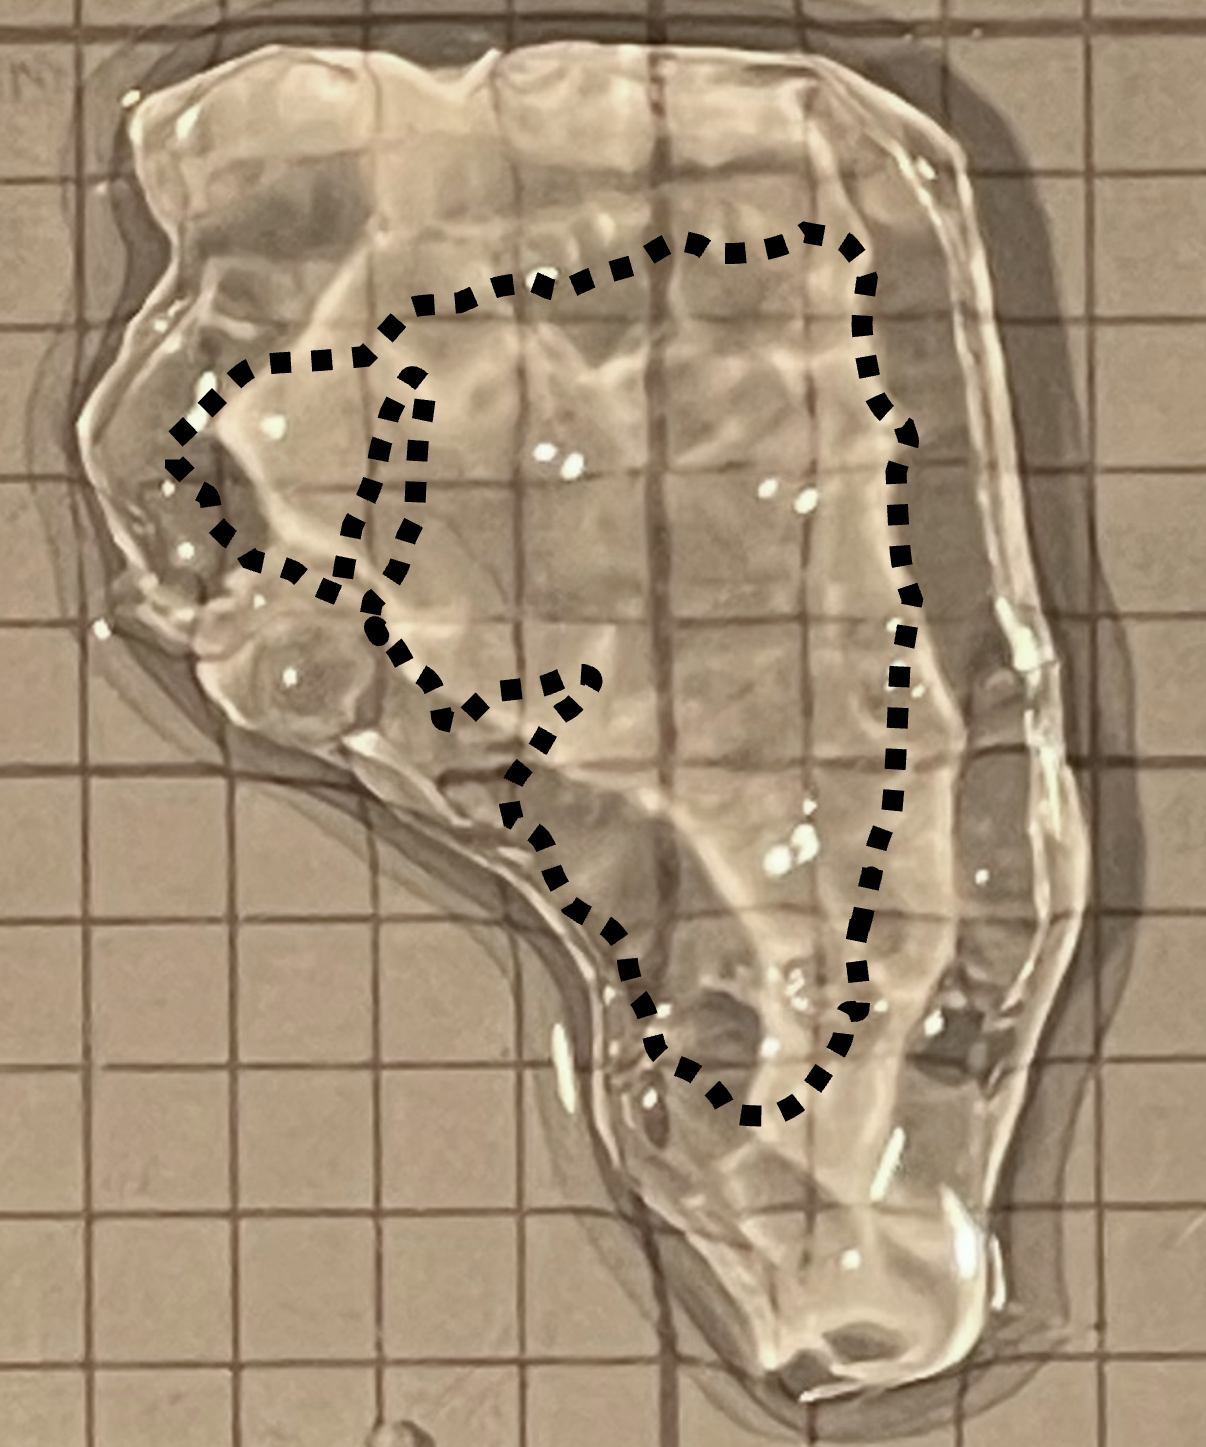
\includegraphics[width=1\linewidth]{Images/CLARITY_Overlay.png}
        \caption{\textbf{Tissue expansion of 400 $\mu$m CLARITY leporine LV sample.} $2 mm^2$ grid background for scale.}
    \end{subfigure}
    ~
    \begin{subfigure}[t]{0.45\textwidth}
        \centering
        \includegraphics[width=1\linewidth]{Images/CUBIC_Overlay.png}
        \caption{\textbf{Tissue expansion of 400 $\mu$m CUBIC-L/RA leporine LV sample.} $1 mm^2$ grid background for scale.}
    \end{subfigure}
    \caption{\textbf{Surface area tissue expansion comparison of CLARITY and CUBIC-L/RA processes.} Perimeter of tissue prior to clearing shown as black dotted outline. Outlines to scale With background grids.}
    \label{fig:enter-label}
\end{figure}


Expansion coefficient of cleared left ventricle section width was determined for 8 LV section samples that underwent CUBIC-L/RA clearing (4 scar, 4 healthy). The width measured in each sample was measured from the endocardial side of each section with the epicardium faced flat onto the petri to the best of our ability. The endocardium face of the tissue section faces perpendicular to the camera in the petri dish. The average axial CE for the entire sample set (as well as the sub-populations of scarred and healthy tissues) were then calculated along with the Standard Deviations observed in each data set. These results were plotted in Figure 3.6:  


\begin{figure}[H]
    \centering
    \begin{tikzpicture}
        \begin{axis}
        [
        scale = 1,
        ytick={1,2,3},
        yticklabels={Overall,Healthy, Scar},
        boxplot/box extend=0.25,
        ]

\addplot+[boxplot] 
            table [y index=0] {Data/CUBIC_Overall.tex}
            [above]
            node at
              (boxplot whisker cs:\boxplotvalue{lower whisker},1)
              {\pgfmathprintnumber{\boxplotvalue{lower whisker}}}
            node at
              (boxplot box cs: \boxplotvalue{median},-1)
              {\pgfmathprintnumber{\boxplotvalue{median}}}
            node at
              (boxplot whisker cs:\boxplotvalue{upper whisker},1)
              {\pgfmathprintnumber{\boxplotvalue{upper whisker}}}
            ;
        
        
\addplot+[boxplot]
            table [y index=0] {Data/CUBIC_Healthy.tex}
            [above]
            node at
              (boxplot whisker cs:\boxplotvalue{lower whisker},1)
              {\pgfmathprintnumber{\boxplotvalue{lower whisker}}}
            node at
              (boxplot box cs: \boxplotvalue{median},-1.5)
              {\pgfmathprintnumber{\boxplotvalue{median}}}
            node at
              (boxplot whisker cs:\boxplotvalue{upper whisker},1)
              {\pgfmathprintnumber{\boxplotvalue{upper whisker}}}
            ;
        
\addplot+[boxplot] 
            table [y index=0] {Data/CUBIC_Scar.tex}
            [above]
            node at
              (boxplot whisker cs:\boxplotvalue{lower whisker},1)
              {\pgfmathprintnumber{\boxplotvalue{lower whisker}}}
            node at
              (boxplot box cs: \boxplotvalue{median},1)
              {\pgfmathprintnumber{\boxplotvalue{median}}}
            node at
              (boxplot whisker cs:\boxplotvalue{upper whisker},1)
              {\pgfmathprintnumber{\boxplotvalue{upper whisker}}}
            ;
        
        
        \end{axis}
    \end{tikzpicture}
    \caption{\textbf{Axial width expansion coefficient of CUBIC cleared LV sections.} Median, upper and lower quartiles, max and min extrema shown (N, overall = 8; n, scar = 4, n; healthy = 4). Data outliers shown as individual data points.}
    \label{fig:enter-label}
\end{figure}

Overall, the average CE for CUBIC-L/RA cleared samples ($\pm {SD}$) was found to be 1.01$\pm {0.06}$. In the subpopulations of LV sections from healthy and scarred hearts, the average Coefficients of Expansion for tissue surface area were seen at 1.01\(\pm {0.08}\) and 1.02\(\pm {0.04}\) respectively. Coefficients of Variation for overall, MI, and healthy heart samples were calculated and rounded up to be 5.94\%, 3.92\%, and 7.92\% respectively. This confirms the average scar and healthy tissue CE values can be utilized in expansion calculations across all tissues in their respective subpopulations. The average overall CE can also be used across all samples as the difference between the average scar and healthy tissue CE was sufficiently negligible for the overall average to remain a valid estimate for all CUBIC-L/RA cleared tissues.

CUBIC-L/RA tissue expansion was confirmed to be extremely minor in sliced cardiac tissue once fully immersed in CUBIC-RA. While slight expansion was seen to occur after exposure to CUBIC-L, the tissue would subsequently contact roughly back to its original size when immersed in CUBIC-RA, with minor differences in orientation occurring in the process. This was confirmed by calculation of a surface area expansion coefficient as being approximately 0.93 for a CUBIC-L/RA 0.4 mm slice and an average axial width expansion coefficient for LV sections. This indicates minimal changes occurred to the samples after clearing with minor difference of attributable to errors and bias encountered when measuring the recorded images. Measurement of LV sections after clearing was particular challenging due to the reduced rigidity of the sample making orientation of the tissues back to their pre-clearing positions for photo documentation more difficult and prone to error. As such, it is determined that the expansion coefficient is not required for analysis of tissue structures within these samples as the change in distance prior to clearing is negligible compared to after clearing.

\subsection{Tissue Transparency}

Highly effective tissue clearing and sample mounting are required in the pipeline to justify use in research and clinical settings. The ability of the pipeline to render cardiomyocytes transparently clear and for the mounting materials to have minimal impact on the transmission of light must be examined. This will confirm that these components of the created imaging pipeline provides sufficient tissue clearing and light transmittance ability compared to other established methods. To this end, the transmittance of light through cleared mounted tissues was examined and compared to transmittance achieved in control samples. Samples containing a variety of Refractive Index matching solutions were also examined to verify their continued use in the imaging protocols. 

\subsubsection{\textit{Methodology}}

Spectroscopic analysis was performed using a spectrofluorometer (HORIBA, Duetta-1621) on multiple cleared left ventricle tissue slices and tissue sections mounted inside custom 3D printed spacer mounts and optical glass cuvettes, respectively. Tissue mounting protocols are provided in Chapter 4. All sliced samples were left to Refractive Index match via immersion in EasyIndex\textrademark for 1 day while all LV section samples were left to immerse in CUBIC-RA for 7 days prior to spectrometer measurement. 

Percent Light Transmission through the mounted samples were recorded in 1 mm increments from 400 nm to 650 nm light wavelengths.  In addition to cleared samples, two uncleared LV tissue slices (0.4 mm and 2.0 mm) as well as one uncleared LV tissue section were also mounted and immersed in their respective RI matching solutions in identical fashion to the cleared samples. 

To establish control baselines for light transmittance data obtained from these mounted tissue samples, multiple 'blank' samples were recorded in tandem with each mounted sample. Four quartz slide custom mounts (0.4 mm, 0.5 mm, 1 mm, 2 mm) containing no sample inside were assembled and filled with EI solution. 

For the CUBIC-L/RA cleared samples, one 'blank' optical glass cuvette was filled with CUBIC-RA solution for use as a control sample. All data was acquired following the protocols set by the spectrofluorometer user manual and software for safe, optimal device performance [].

\subsubsection{\textit{Mounted CLARITY Results}}

To showcase the improvement in transmission possible with the CLARITY protocol utilized in the imaging pipeline, Light Transmittance from cleared 0.4 mm and 2.0 mm thick LV cardiac tissue slices were compared to samples that underwent no clearing protocol after perfusion and fixation. These recorded samples and were plotted across 400 to 650 nm light wavelengths and are shown in Figure 3.7(a-b) below:

\begin{figure}[H]
    \centering
    \begin{subfigure}[t]{0.9\textwidth}
    \centering
    \begin{tikzpicture}
    
    \begin{axis}[
            ymajorgrids,
            xmajorgrids,
            scale= 1.2,
            width = 12cm,
            height = 7cm,
            ylabel={Transmission (\%)},
            xlabel={Wavelength (nm)},
            xmin = 390, xmax = 660,
            ymin = -10, ymax = 105,
            legend style={at={(0.7,0.2)}, 
            anchor=north}
            ]
        \addplot+[
            const plot,
            color=blue,
            mark=square,
            mark size = 3pt,
            error bars/.cd,
                x dir=both, x fixed = 1,
                y dir=both, y fixed = 4.5
            ]
            table [ x index=0, y index=3]{Data/400um_UNCLEARED_2.dat};%400um_CLARITY_UNCLEARED_TRANSMISSION.dat};
        \addplot+[
            color=red,
            mark=o,
            mark size = 3pt,
            error bars/.cd,
                x dir=both, x fixed = 1,
                y dir=both, y fixed = 4.5
            ]
            table [x index=0, y index=2] {Data/400um_CLEARED_2.dat};%CLARITY_Transmission.dat};
        \legend{0.4 mm Uncleared, 0.4mm Cleared}
        \end{axis}
    \end{tikzpicture}
    \caption{\textbf{Percent light transmission of mounted 0.4mm CLARITY sliced samples.} Light transmittance normalized to control 400um Mount, filled with EI solution.}    
    \label{fig:enter-label}
    \end{subfigure}
    \medskip
    
    \begin{subfigure}[t]{0.9\textwidth}
    \centering
    \begin{tikzpicture}
    \begin{axis}[
            ymajorgrids,
            xmajorgrids,
            scale= 1.2,
            width = 12cm,
            height = 7cm,
            xlabel={Wavelength (nm)},
            ylabel={Transmission (\%)},
            xmin = 390, xmax = 660,
            ymin = -10, ymax = 105,
            legend style={at={(0.725,0.2)}, 
            anchor=north}
            ]
        \addplot+[
            const plot,
            color=blue,
            mark=square,
            mark size = 3pt,
            error bars/.cd,
                x dir=both, x fixed = 1,
                y dir=both, y fixed = 4.5
            ]
            table [ x index=0, y index=3] {Data/2mm_CLARITY_UNCLEARED_TRANSMISSION.dat};
        \addplot+[
            color=red,
            mark=o,
            mark size = 3pt,
            error bars/.cd,
                x dir=both, x fixed = 1,
                y dir=both, y fixed = 4.5
            ]
            table [x index=0, y index=2] {Data/2mm_CLARITY_TRANSMISSION.dat};
        \legend{2 mm Uncleared, 2 mm Cleared}
        \end{axis}
    \end{tikzpicture}
    \caption{\textbf{Percent light transmission of mounted 2.0mm CLARITY sliced samples.} Light transmittance normalized to control 2mm mount, filled with EI solution.}    
    \label{fig:enter-label}
    \end{subfigure}
    \medskip
    
    \caption{\textbf{Comparison of percent light transmission of mounted cleared and uncleared sliced cardiac tissue samples.}  Spectrofluorometer \% transmittance accuracy: $\pm$ 4.5\%, wavelength emission accuracy: $\pm$ 1 nm []. Data presented downsampled from 1 nm increment to 5 nm for clarity.}    
    \label{fig:enter-label}
\end{figure}

Percent light transmission across 0.4 mm and 2.0 mm mounted, CLARITY cleared samples were recorded and presented in Figure 3.5 for comparison of transmittance across thickness examined in this project. Percent transmittance across these samples were normalized to the blank mounts of corresponding thickness (0.4 mm and 2.0 mm respectively). 0.5 mm and 1.0 mm cleared samples were not analysed as part of this series due to the limited sample inventory available. 


\begin{figure}[H]
    \centering
    \begin{tikzpicture}
    \begin{axis}[
            ymajorgrids,
            xmajorgrids,
            xmin = 395, xmax = 655,
            ymin = 85, ymax = 100.25,
            scale= 1.2,
            width = 12cm,
            height = 7cm,
            ylabel={Transmission (\%)},
            xlabel={Wavelength (nm)},
            legend style={at={(0.8,0.2)}, 
            anchor=north}
            ]
        
        \addplot+[
            color=orange,
            mark=diamond,
            mark size = 5pt
            ]
            table [x index=0, y index=2] {Data/400um_CLARITY_Transmission.dat};
     
        \addplot+[
            color=blue,
            mark=x,
            mark size = 5pt
            ]
            table [x index=0, y index=2] {Data/2mm_CLARITY_Transmission.dat};
            \legend{0.4mm, 2.0mm}
        \end{axis}
    \end{tikzpicture}
    \caption{\textbf{Percent light transmission of mounted 0.4 and 2.0 mm CLARITY cleared, unstained sliced samples.} Tissue sample light transmittance normalized to respective thickness control mounts filled with EI solution. Spectrofluorometer\% transmittance accuracy: $\pm$ 4.5\%, wavelength emission accuracy: $\pm$ 1 nm []. Manufacturer stated error margins omitted from plot for clarity. Data presented downsampled from 1 nm increment to 5 nm for clarity}
    \label{fig:enter-label}
\end{figure}

Likewise, percent light transmittance across 0.5, 1.0, and 2.0 mm blank mounts were recorded and normalized with respect to the 0.4 mm blank mount sample. This allows changes in light transmittance as internal mount volume increases to be examined in detail across the utilized light spectrum. The data obtained from these light transmittance recordings are shown in Figure 3.9.
    
\begin{figure}[H]
    \centering
    \begin{tikzpicture}
    \begin{axis}[
            ymajorgrids,
            xmajorgrids,
            scale= 1.2,
            width = 12cm,
            height = 7cm,
            xmin = 390, xmax = 660,
            ymin = 92.5, ymax = 100.25,
            ylabel={Transmission (\%)},
            xlabel={Wavelength (nm)},
            legend style={at={(0.8,0.5)}, 
            anchor=north}
            ]
        
        \addplot+[
            color=red,
            mark=o,
            mark size = 3pt,
            %error bars/.cd,
                %x dir=both, x fixed = 1,
                %y dir=both, y fixed = 4.5
            ]
            table [x index=0, y index=1] {Data/0.5mmBlankData.dat};
        \addplot+[
            color=green,
            mark=square,
            mark size = 3pt,
            %error bars/.cd,
                %x dir=both, x fixed = 1,
                %y dir=both, y fixed = 4.5
            ]
            table [x index=0, y index=1] 
            {Data/1mmBlankData.dat};
        \addplot+[
            color=blue,
            mark=x,
            mark size = 5pt,
            %error bars/.cd,
                %x dir=both, x fixed = 1,
                %y dir=both, y fixed = 4.5
            ]
            table [x index=0, y index=1] 
            {Data/2mmBlankData.dat};
            \legend{0.5mm, 1.0mm, 2.0mm}
        \end{axis}

        
    \end{tikzpicture}
    \caption{\textbf{Percent light transmission of mounted control samples filled with EI solution.} Control light transmittance normalized to control 0.4 mm mount filled with EI solution. Spectrofluorometer\% transmittance accuracy: $\pm$ 4.5\%, Wavelength Emission Accuracy: $\pm$ 1 nm []. Manufacturer stated error margins omitted from plot for clarity. Data presented downsampled from 1 nm increment to 5 nm for clarity.}
    \label{fig:enter-label}
\end{figure}

Tissue transparency experiments verified the ability of CLARITY  to sufficiently clear sliced tissues for light sheet imaging and the ability of quartz glass to match the RI of the EasyIndex immersion solutions. Percent light transmittance recorded remained above 90\% for CLARITY cleared samples in all examined wavelengths of light. In contrast, a significant decline in transmittance was seen to occur in CUBIC-L/RA samples, with light transmittance only being comparable to CLARITY in wavelengths greater than 607 nm. While transmittance in wavelengths under 607 nm was poorer in CUBIC-L/RA samples compared to CLARITY samples, the transmittance was still greater in all wavelengths compared to the uncleared control LV section immersed in CUBIC-RA. 

Experiments examining transmittance of light across EI solution filled, custom fabricated mounts containing no samples confirmed that increasing the optical path length inside the custom mount did not noticeably impact the transmission of light when compared to transmission across the thinnest mount (0.4 mm). Across the entire examined wavelength range, light transmission compared to the 0.4 mm control remained above 92\%$\pm$ 4.5\% in all mount thicknesses. This match in transmission increases to >99\%$\pm$ 4.5\% match to the 0.4 mm mount in wavelengths above 422 nm. Increasingly large drops in percent transmission are seen in wavelengths below 420 nm, with the drop increasing from 0.42\% in the 0.5 mm mount to 5.96\% in the 2.0 mm mount. This slight decline in transmission at lower wavelengths is roughly identical to the drop in transmittance seen in recording taken of mounts containing samples. This suggests this decline at the lowest wavelengths examined is inherit to the quartz glass used in sample mount as prior transmission tests on pure quartz indicate a sudden decline in transmission does occur at this wavelength range [].


\subsubsection{\textit{CUBIC-L/RA Results}}

Light transmission percentage was recorded for a cleared LV tissue section sample. An uncleared LV cardiac section was also recorded to show the improvement in transmission possible with clearing protocol compared to an uncleared LV section.  Percent light transmission across an empty cuvette containing only CUBIC-RA solution was used to normalize cleared and uncleared sample data against. These recorded light transmissions were plotted across the light wavelength range examinable by the mesoSPIM laser engine and is shown in Figure 3.10 below: 

\begin{figure}[H]
    \centering
    \begin{tikzpicture}
    \begin{axis}[
            ymajorgrids,
            xmajorgrids,
            scale= 2,
            width = 8cm,
            height = 5cm,
            ylabel={Transmission (\%)},
            xlabel={Wavelength (nm)},
            xmin = 390, xmax = 660,
            ymin = 0, ymax = 100,
            legend style={at={(0.3,0.9)}, 
            anchor=north}
            ]
       \addplot[
            color=red,
            mark=o,
            mark size = 3pt,
            error bars/.cd,
                x dir=both, x fixed = 1,
                y dir=both, y fixed = 4.5
            ]
            table [x index=0, y index=1] {Data/CUBIC_2.dat};%Transmission.dat};
        \addplot[
            color=blue,
            mark=x,
            mark size = 5pt,
            error bars/.cd,
                x dir=both, x fixed = 1,
                y dir=both, y fixed = 4.5
            ]
            table [x index=0, y index=1] {Data/CUBIC_UNCLEARED_Transmission.dat};
        \legend{Cleared LV Section, Uncleared LV Section}
        \end{axis}
    \end{tikzpicture}
     \caption{\textbf{Percent light transmission of LV section samples with and without CUBIC-L/RA clearing.} Light transmittance normalized to 0.4 mm control mounted inner cuvette filled with CUBIC-RA solution. Spectrofluorometer \% transmittance accuracy $\pm$ 4.5\%, wavelength emission accuracy $\pm$ 1 nm. Manufacturer stated error margins omitted from plot for clarity. Data presented downsampled from 1 nm increment to 5 nm for clarity.}
    \label{fig:enter-label}
\end{figure}

Tissue transparency experiments verified the ability of CUBIC-L/RA to sufficiently clear tissues for light sheet imaging and the ability of  optical glass to match the RI of CUBIC-RA immersion solution. Light Transmittance in CUBIC-L/RA samples was found to decline at a relatively linear rate as the wavelength of light lowered. This low transmittance indicates a sharp increase in light scattering inside the sample, which will increase background noise and lower the resolution in light sheet imaging when performed using lasers sources approaching the violet end of the visible spectrum of light (500-400 nm).  This result confirms prior publications reports of the lower quality of CUBIC-L/RA clearing compared to CLARITY, which retains high transmittance across the wavelengths of observable light []. These results also show that the protocol remains viable for imaging at higher wavelengths, which shows light transmittance of CUBIC-L/RA is comparable to CLARITY cleared samples at wavelengths $\geq590$ nm and remaining above 50\% transmittance at wavelengths $\geq510$ nm.

This is also corroborated by the images obtained by the mesoSPIM microscope of fluorescently stained CUBIC-L/RA samples, which decreased in quality and resolution as the light emitted by dyes lowered in wavelength (see Chapter 5.2). 

\subsection{Tissue Structural Assessment}

To confirm the condition of the tissue remains viable for use in histology and morphological examination, the structure of tissue after clearing must be shown to be in good condition using an alternative microscopy technique other than LSM. Use of an second, more well established microscopy system (such as multi-photon microscopy) will provide an objective look at the tissue structure that could otherwise be concealed or hidden by unforeseen issues or flaws that existed in the developing imaging pipeline at the time.

The most serious form of structural damage encountered in prior research was the breaking apart of the myocardium's dense cell volume (fibre delamination) []. This structural change presents as large voids of space between the normally densely packed strands of cardiac muscle. An example of this damage to structure seen in prior publications using other types of clearing protocols are shown below:

\begin{figure}[H]
\centering
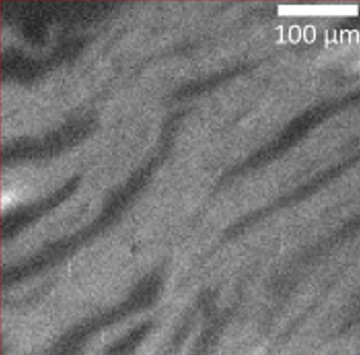
\includegraphics[width=0.5\linewidth]{Images/Camilla Picture.jpg}
\label{fig:enter-label}
\caption{\textbf{Alterations to cardiac tissue structure encountered in prior tissue clearing research [].} Tissue cleared using the uDISCO dehydration tissue clearing protocol by Dr. Camilla Olianti. Dark Regions Signify Voids in Tissue From Fibre Delamination.}
\end{figure}

This damage is the key feature that will be searched for in samples imaged using the 3P microscope. Should such damage in cleared samples be no more prevalent than it is in uncleared control sample, it will confirm the clearing methods remain valid for use in the structural imaging pipeline being established. Comparison between the CLARITY and CUBIC-L/RA samples imaged with the 3P system will also allow their structural preservation ability to be compared and contrasted, which can aid future users of the pipeline in deciding which method they should use in their research.

\subsubsection{\textit{Methodology}}
 Multi-photon microscopy was utilized to image small regions of uncleared, CLARITY cleared, and CUBIC-L/RA cleared cardiac tissue samples with lateral resolution of xx um. Concurrently to this project, a separate project in the same research group saw the assembly and characterization of a multi-photon system in an adjacent lab space. Imaging using this system was performed by doctoral candidates Lewis Williamson and Ahmed Elnageh under the guidance of Dr. Caroline Muellenbroich. 
 
 Utilizing 2-photon and 3-photon microscopy has the benefit of both confirming the preservation of tissue structure after clearing as well as verifying the quality of images acquired of samples using the mesoSPIM light sheet microscopy technique beforehand. To accomplish this, mounted CLARITY samples stored inside custom 3D printed mounts must be removed from the mount as the working distance of the 2/3-photon system is unable to pass through the 1 mm thick quartz slides.
 
 To remove samples from the custom mounts, cured silicon sealant is removed from the edges of the quartz slides using pipette tips and the sides of the printed mount are gently pulled apart to pull the slides out of the internal spacer. The process will leak out all contained RIMS, so precautions such as gloves, ethanol cleaning solution, and paper towels are required to safely collect all drained solution and prevent chemical contamination on surfaces or skin contact.

 After cleaning drained solution, the tissue between the quartz slides is gently removed by lifting the top slide off of the sample and using a small, rounded paintbrush to lift the sample off of the bottom slide. Once full removed from both slides, the sample is placed flat atop a 25 mm x 100 mm glass cover-slip. Tweezers are used to remove any loose fibres from the paintbrush left behind on the sample during the transfer and used to orient the sample on the cover slip to match the orientation of the sample when it was inside the mount. An example of a CLARITY cleared tissue slice removed and placed onto a cover-slip using this method is shown in Figure 3.9(a). After orienting the sample, a single drop of EasyIndex solution is dropped atop the sample with a pipette. A second  glass cover-slip (25 mm x 50 mm) is then placed atop the sample ensuring no bubbles form between the cover-slip and tissue surface (shown in Figure 3.9(b)). 

\begin{figure}[H]
\centering
\begin{subfigure}[t]{0.475\textwidth}
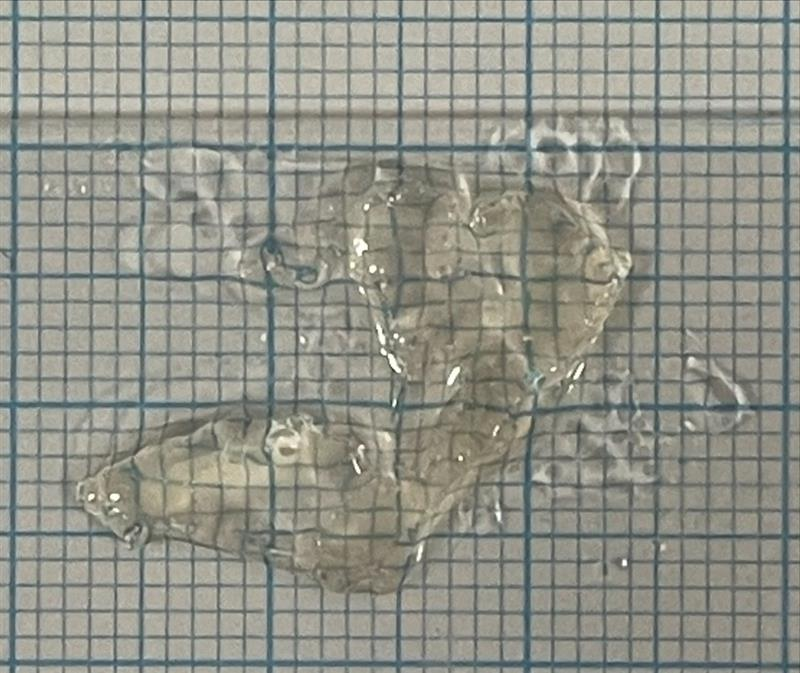
\includegraphics[width=1\linewidth]{Images/Figure3.12a.jpg}
\caption{\textbf{CLARITY sample removed from mount, placed onto cover-slip before paintbrush reorientation}}
\label{fig:enter-label}
\end{subfigure}
~
\begin{subfigure}[t]{0.475\textwidth}
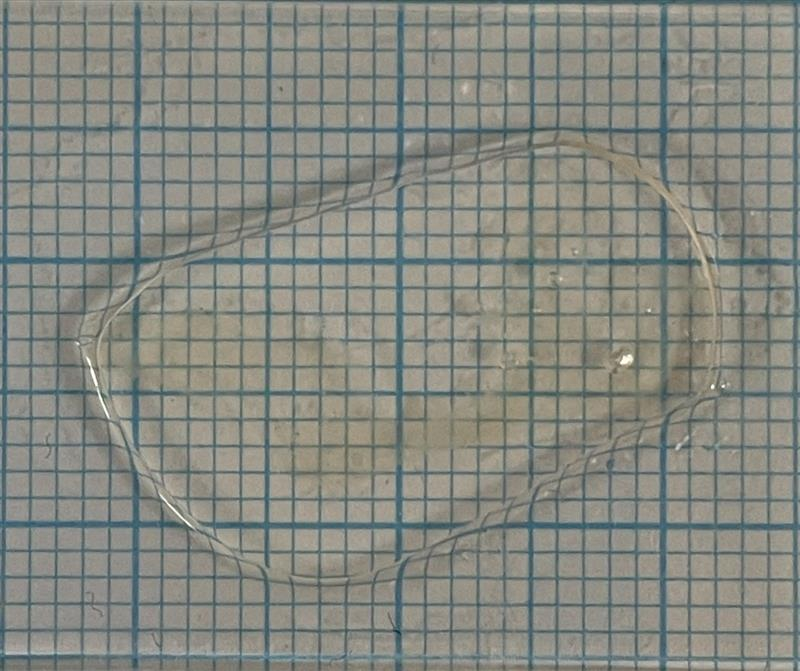
\includegraphics[width=1\linewidth]{Images/Figure3.12b.jpg}
\caption{\textbf{CLARITY sample after reorientation, placement of easy index drop and second cover slip on top.}}
\label{fig:enter-label}
\end{subfigure}
\caption{\textbf{CLARITY sample preparation for Multi-photon imaging after removal from custom 3D printed mount.} 1 $mm^2$ grid background for scale.}
\end{figure}
 

\subsubsection{\textit{Results}}

Images of myocardial tissue across a 250 micron x 250 micron FOV were captured of cleared and uncleared cardiac samples using the multi-photon microscope system. These images are shown in a side by side comparison in the following Figure:

\begin{figure}[H]
\centering
\begin{subfigure}[t]{0.475\textwidth}
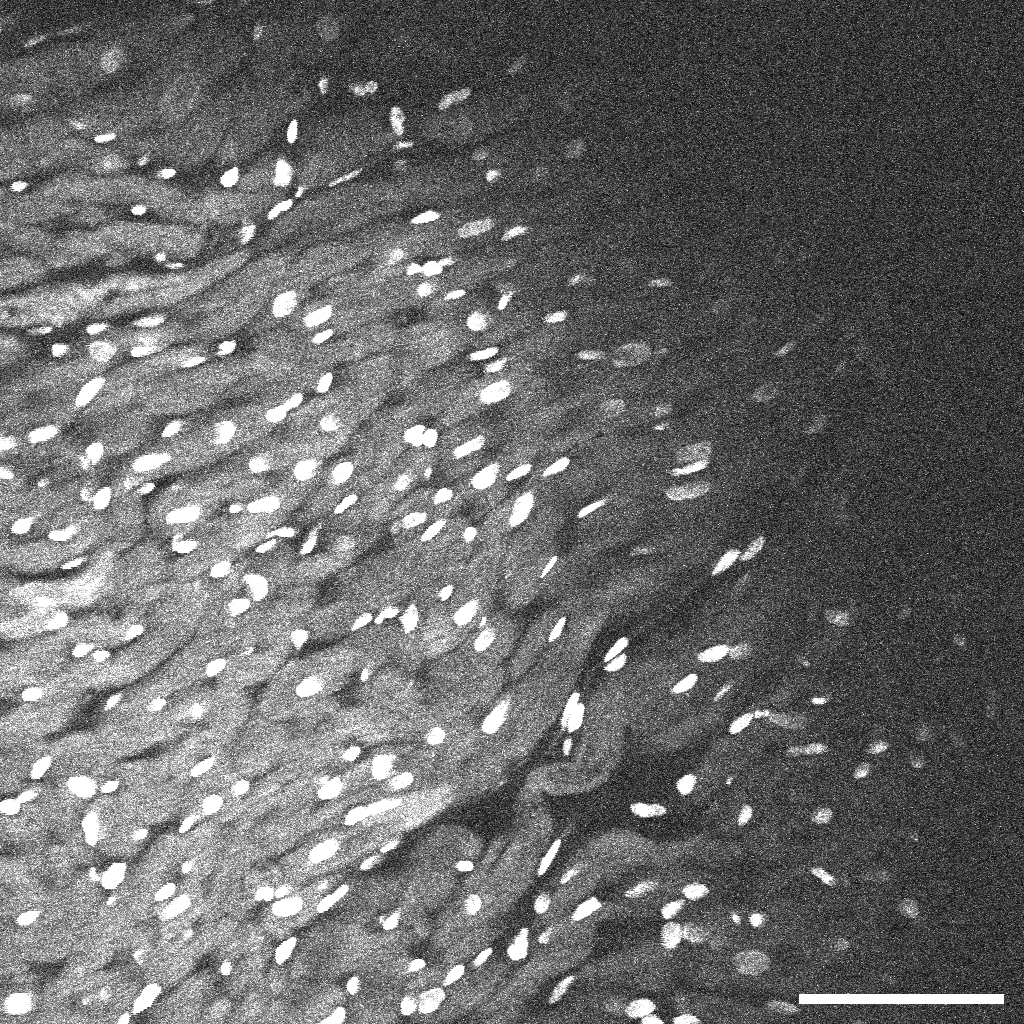
\includegraphics[width=1\linewidth]{Images/Uncleared_Structure.png}
\caption{\textbf{3P image of uncleared tissue structure.} 405 nm excitation channel, cell nuclei stained using DAPI.}
\label{fig:enter-label}
\end{subfigure}
~
\begin{subfigure}[t]{0.475\textwidth}
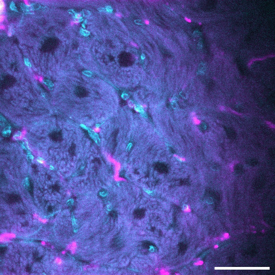
\includegraphics[width=1\linewidth]{Images/CLARITY_3P.png}
\caption{\textbf{3P image of CLARITY cleared tissue structure.} WGA/AF-488 fluorescence highlighted in cyan, anti-TH fluorescence highlighted in magenta.}
\label{fig:enter-label}
\end{subfigure}
\medskip

\begin{subfigure}[t]{0.475\textwidth}
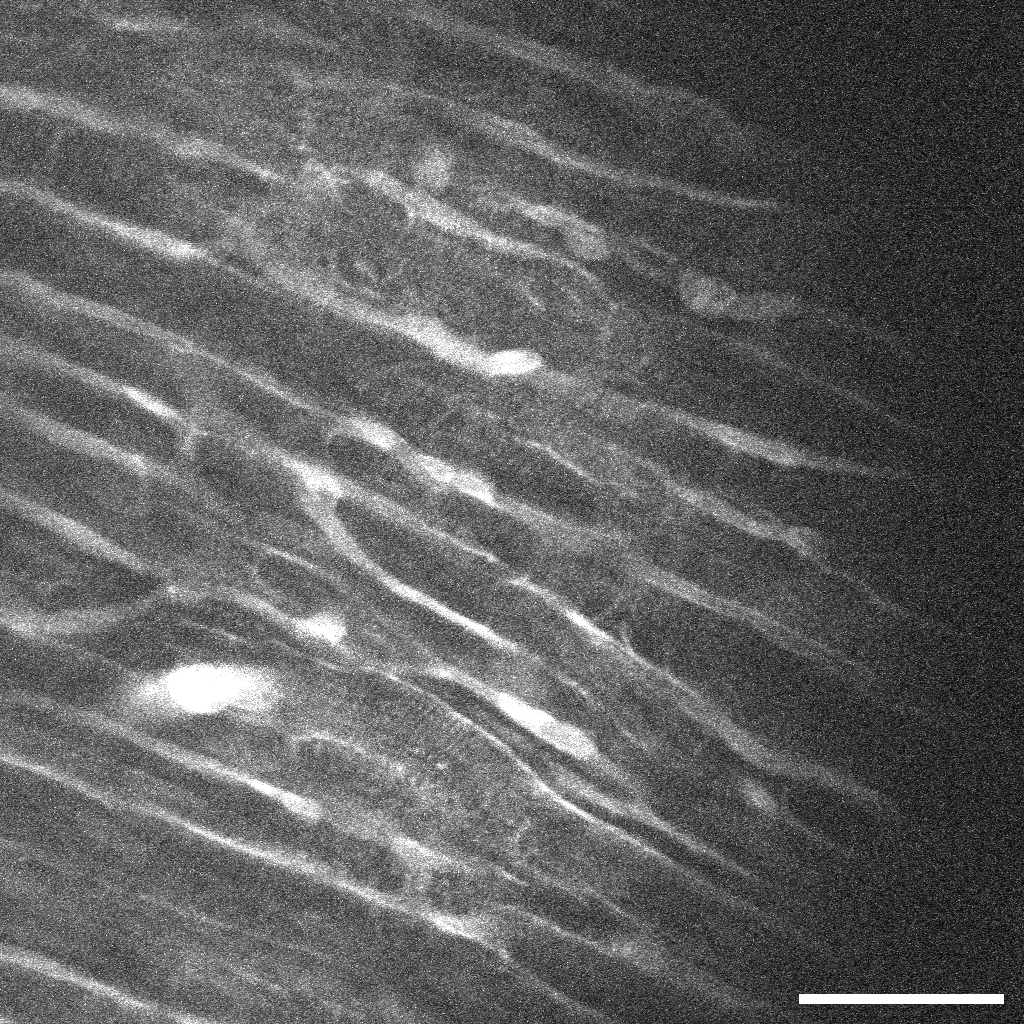
\includegraphics[width=1\linewidth]{Images/CUBIC_Structure.png}
\caption{\textbf{2P image of CUBIC-L/RA cleared tissue structure.} 647 nm excitation channel, cell membranes stained using WGA-647.}
\label{fig:enter-label}
\end{subfigure}
\caption{\textbf{Comparison of myocardial tissue structure in cleared and uncleared leporine sliced tissue samples.} Multi-photon microscopy images acquired by Lewis Williamson, Ahmed Elnageh. Scale bar = 50 microns.}
\end{figure}

Qualitative analysis of the images upon acquisition indicated that there was negligible change in structure between the three images. No significant delamination, as seen in dehydrating methods of tissue clearing performed in other published research (See Figure 3.13), were seen in the samples imaged as shown in Figure 3.13 (b-c). Negligible space was seen between adjacent cells in the cardiac tissue. 

The only significant alterations encountered were found at the edges of the tissue slices and sections, which were determined to be a direct results of the dissection process physically breaking apart the fibres of the tissue to remove the tissue from the rest of the heart. This damage is unavoidable and mitigated by the use of a Vibratome tissue slicer in the case of tissue slices and by the use of surgical scissors for LV tissue sections. Sectioning and slicing damage remained consistent across samples indicating damage did not spread as a result of either clearing protocol.

Due to time constraints and limited data availability, quantitative analysis to confirm these finding could not be performed. However, the qualitative results seen here, combined with prior published structural preservation studies performed using CLARITY and CUBIC-L/RA cleared cardiac samples, were deemed sufficient enough evidence to proceed with the usage of both clearing protocols in the clearing pipeline. 

\section{Discussion}
The main aim of this series of experiments was to produce an optimized tissue clearing procedure and to categorically confirm the preservation of structural data in samples that undergo this protocol for use in biological, clinical analysis. The results obtained from the experiments described in this chapter confirms that the finalized pipeline protocol described in Chapter 3.1 is fully capable of producing high quality images of ex vivo tissue structure when implemented as part of the overarching tissue imaging pipeline. 


\subsection{Tissue Clearing Discussion}
Throughout the course of tissue slicing, clearing, and analysis, multiple issue arose that made data reliability and accuracy difficult to maintain. Multiple samples had to be discarded or omitted from analysis due to these issue making reliable measurement or analysis nearly impossible. The extended time periods required to complete these protocols make avoidance of such issues imperative for successful implementation of the imaging pipeline, thus these issue were closely examined and documented to aid in future prospects discussions.

\subsubsection{\textit{Slicing Difficulties}}
In tissue slicing, it was found that the more fibrous scarred tissue regions would be far more resistant to precision slicing in the Vibratome. It was not uncommon for the blade to get caught on this tissue and instead of continuing to cut though, would simply pull the entire tissue out of the agar block it was embedded inside. Most samples could be salvaged from these incidents although significant amounts of time and resources were lost in the process, with the partially sliced section of the sample being discarded to ease the slicing process on the remaining tissue. To remedy this issue, steel blades were replaced with ceramic blades, which were able to slice through the scar tissue reliably with minimal difficult compared to the steel blades. As an added precaution, an additional agar block was added behind the agar embedded sample in the Vibratome to add support against the forward movement of the blade, decreasing the possibility of the blade pulling the sample out of the agar mid-slice.

\subsubsection{\textit{CLARITY Protocol Difficulties}}
During tissue clearing experimentation, only 2 session of CLARITY clearing could be completed during the course of this research due to the extremely long time span required to clear tissues using this method. The protocol's complicated procedure also requires 5 intensive days of laboratory work to complete the initial clearing steps before samples can begin the months long washing that requires minimal user interaction to complete. The long time and resource investment just to start the months long protocol was found to be too time consuming to perform multiple times in a short time period for a handful of samples at a time. It was decided instead to perform the session only 2-3 times with each instance clearing the entire inventory of cardiac tissue slices available at once. 

The downside of performing these bulk sample clearing session was that it was extremely difficult to alter the protocol were problems to arise, as they would not be noticeable in most cases until near the end of the half-year washing period. Should a problem emerge, it could effect the entire sample population and render the entire inventory unusable as a consequence.To complicate the matter, any changes to the protocol that is made to correct these issues would require restarting the procedure with a new batch of sliced tissues from scratch, setting back research efforts back 6-8 months in the process as we await to see if the changes made were able to resolve a given issue. 

To prevent such time consuming set backs, great care and precaution was taken during both clearing sessions to follow the established protocol as closely as possible with minimal deviation. The first session was even performed under the direct observation of its creator, Dr. Camilla Olianti, to ensure successful implementation of the clearing process in at least the first instance. As a result of these additional measures, clearing of tissues in both sessions were completed with all tissues sufficiently cleared for imaging to occur.

\subsubsection{\textit{CLARITY Cleared Tissue Curling}}

One of the few complications found in the CLARITY protocol, which impacted a majority of CLARITY cleared samples in the first session and a minority in the second session was slice warping. It was found that after completing the washing step, the cleared tissues were highly susceptible to curling and warping in three dimensions. Examples of this curling seen in both sessions are shown in Figure 3.17 below.


\begin{figure}[H]
    \centering
    
    \begin{subfigure}[t]{0.475\textwidth}
    \centering
    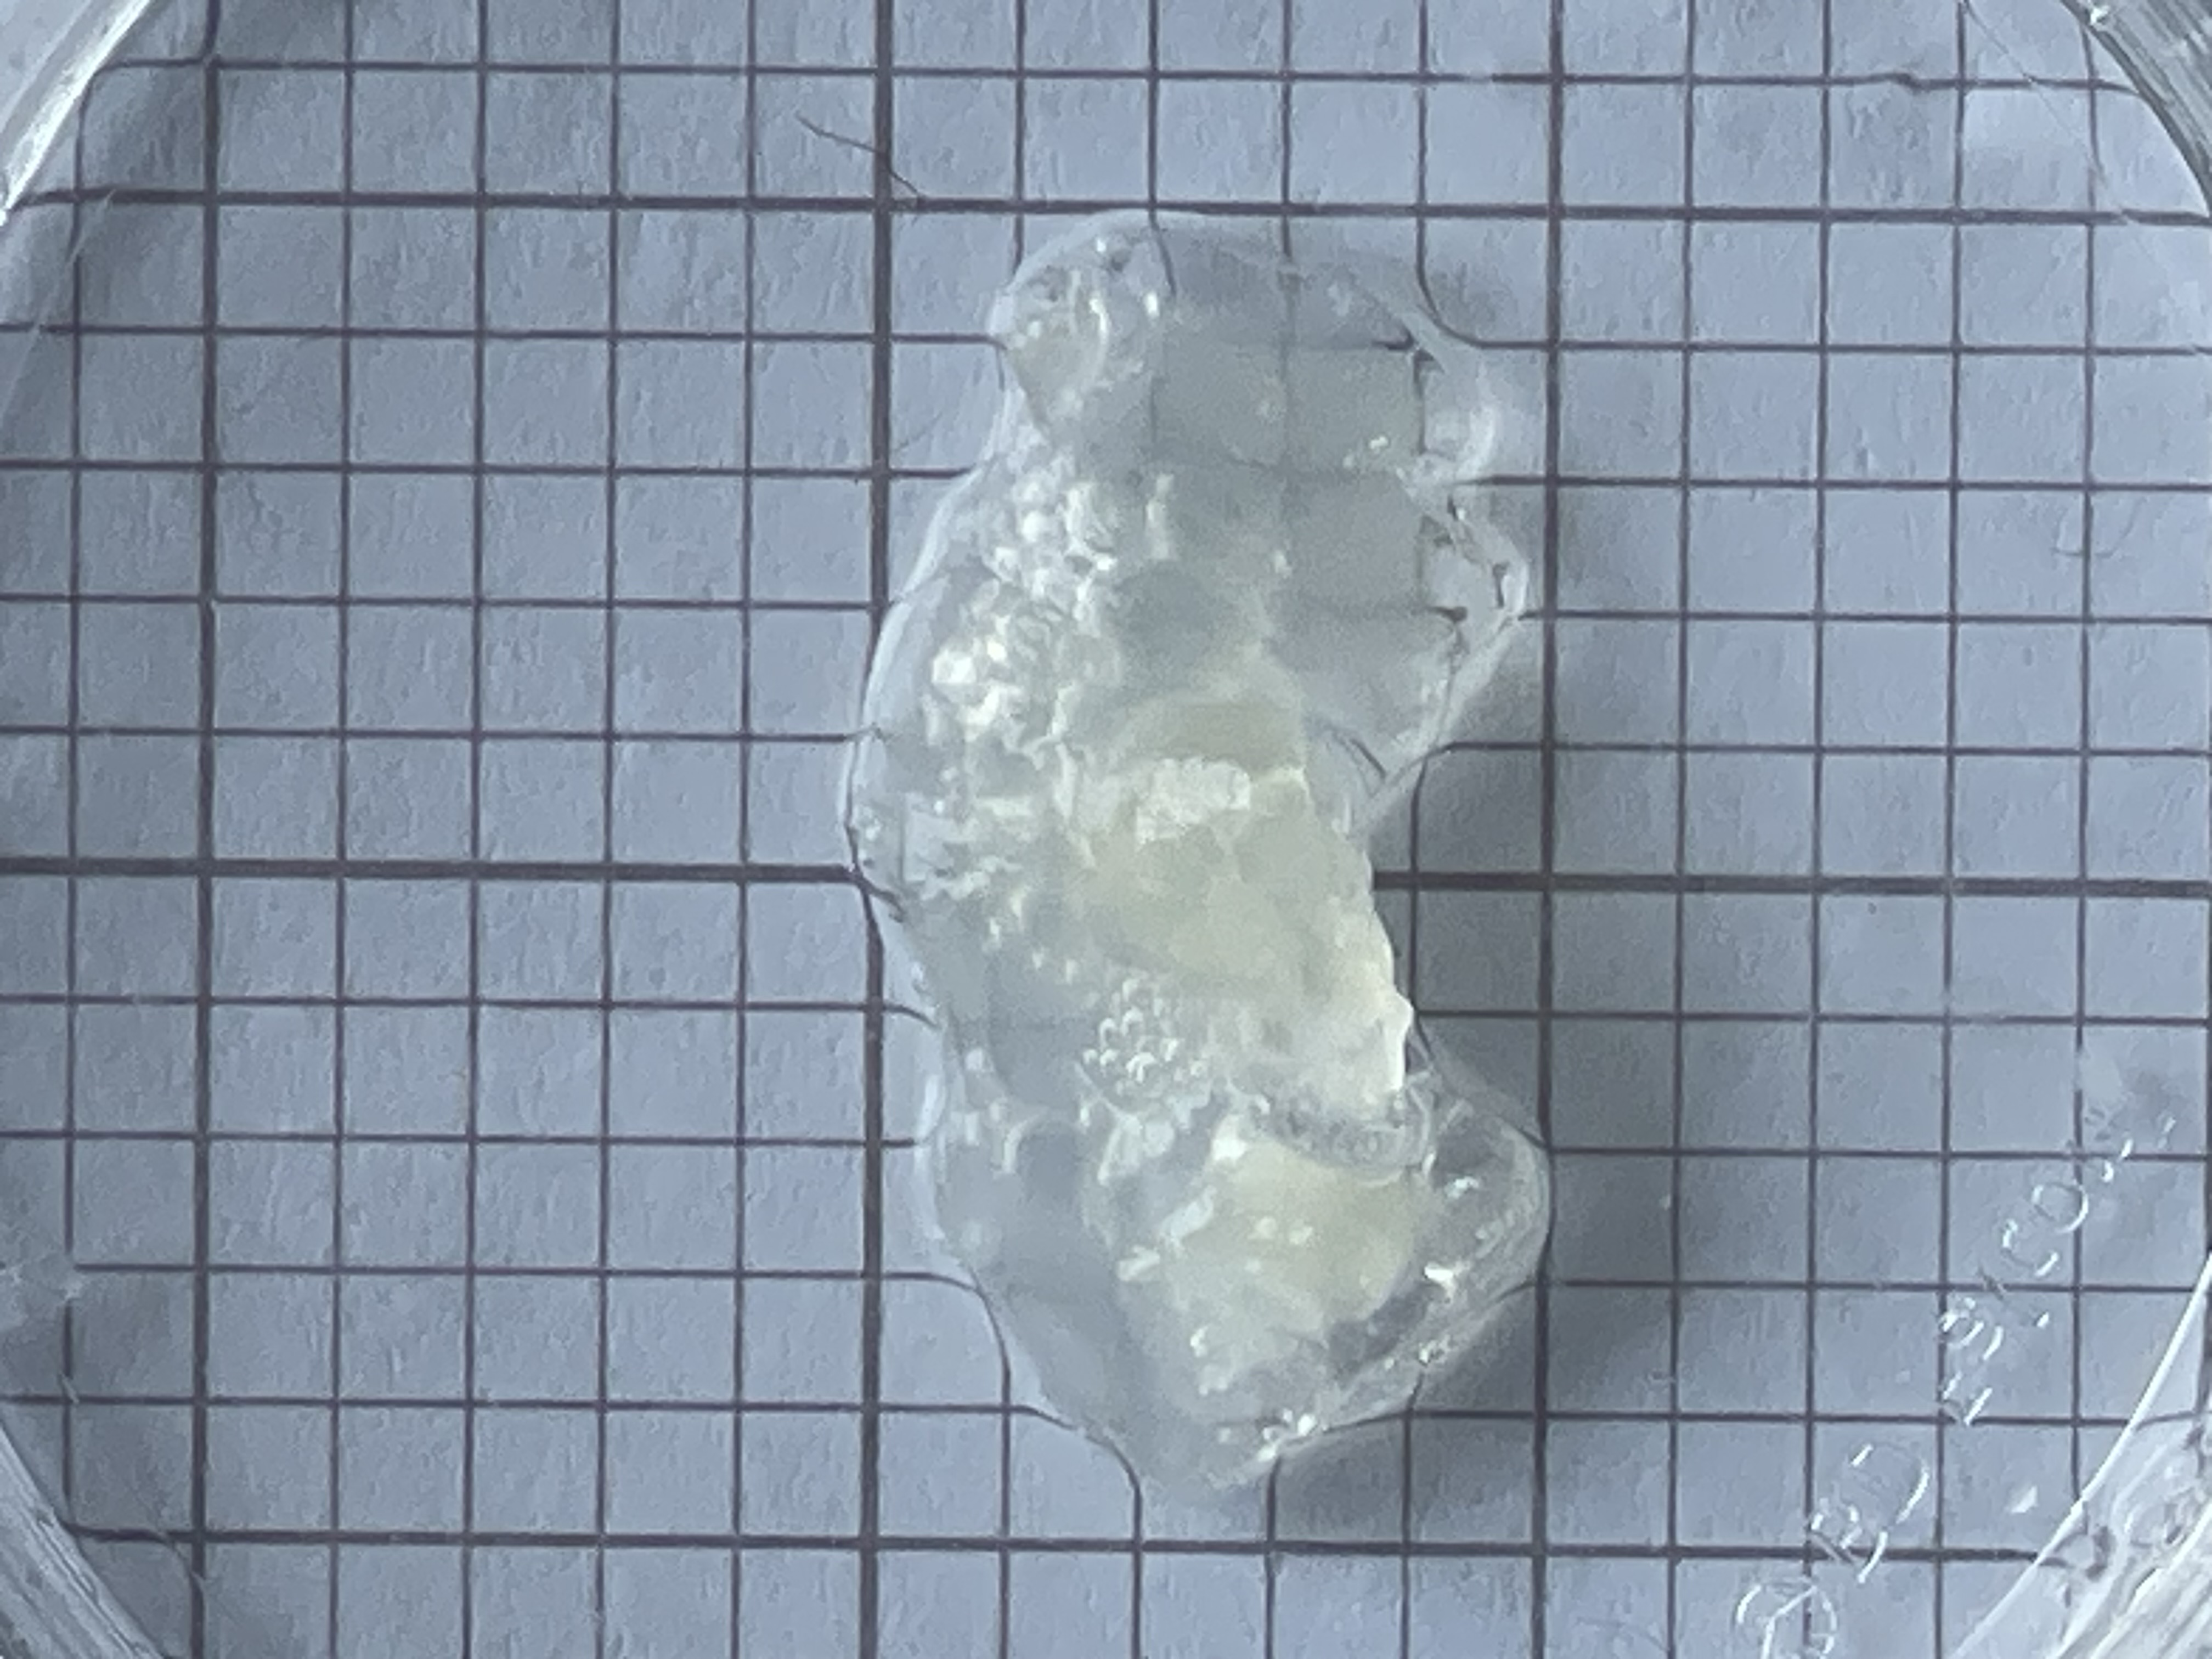
\includegraphics[width=1\linewidth]{Images/FirstSessionWarp.JPG}
    \caption{Tissue curling of CLARITY cleared tissue washed in test tube (first clearing session)}
    \end{subfigure}
    ~
    \begin{subfigure}[t]{0.475\textwidth}
    \centering
    \includegraphics[width=1\linewidth]{Images/SecondSessionWarp.JPG}
    \caption{Tissue curling of CLARITY cleared tissue washed in petri dish (second clearing session)}
    \end{subfigure}
    \medskip
\caption{\textbf{Examples of severe CLARITY sample tissue curling encountered during experimentation.} 1 $mm^2$ grid background for scale.}
    \label{fig:enter-label}
\end{figure}

    
In the first clearing session, samples were stored in 15 mL test tubes for the duration of the washing period. A side effect of this storage method was that many of the samples contoured to match the curve of the tube walls or of the tube's conical end. When removed from these tubes to document expansion, the samples would retain these curled shapes, making lateral expansion documentation impossible to photograph (seen in Figure 3.10(a)). Forcibly flattening thin and healthy cardiac slice samples using pipette tips and slides would allow some to be placed into in a flattened state, but scarred and thicker samples with severe curling could not be flatten without breaking the sample apart in the process.  

To prevent this issue from occurring again, the second session saw the washing step utilize petri dishes instead of test tubes for long term storage. While this change did reduce the occurrence of tissue curling, a minority of samples were still impacted enough to render them unusable for expansion analysis (as seen in Figure 3.10(b)). It is believed these samples contoured to the cylindrical walls of the petri dish, but as these samples were the final samples population to be cleared using CLARITY, there were no further opportunities to test further measures to prevent this curling from occurring. Possible remedies could include washing the samples inside the mounts used for imaging or laying a cover slip of equal diameter to the washing petri dish atop the sample in solution. This would likely prevent any curling from occurring but simultaneously would also extend the washing process by months due to the reduced contact and motion the sample would have in the washing solution. For time limitations this was not attempted in this project but could be tested in future trials as a possible remedy to the issue.

This curling phenomenon caused additional issues when mounting CLARITY samples into the custom designed mount spacers as they made insertion into mounts far more challenging to complete without damaging the sample. Even when uncurled, the tissue would apply pressure on the slides they were placed in as they try to return to their curled states, applying strain against the slides that could cause astigmatisms and aberrations to form in the acquired images as a direct result. This is an issue already inherently present in the design of the sliced tissue imaging mounts (see Chapter 4.3), which is only exacerbated by this additional pressure applied by the uncurled samples. 

\subsubsection{Introduction of CUBIC-RA}
At the start of this project, the use of CUBIC-L/RA was not even considered for use with the cardiac tissue samples. At the time, only CLARITY was being performed and was the only method attempted which had produced viable results. An additional protocol, SHIELD, was also explored as a potential alternative to CLARITY but was quickly abandoned due to poor results and tissue shrinkage results in cleared samples becoming unusable. 

It was during the long washing period of the second round of CLARITY tissue clearing that CUBIC-L/RA was discovered and shown to be a viable alternative to CLARITY. The CUBIC family of hyper-hydrating protocols sacrifices high quality tissue clearing for a significantly reduced processing time and complexity compared to CLARITY (~1 month for a 500 $mm^3$ section of LV wall with CUBIC-L/RA vs ~8 months for a 60 $mm^3$ LV transmural slice). While the reduction in tissue clearing quality would undoubtedly reduce the resolution and penetration of the light sheet into thicker samples, prior results obtained by implementing the protocol with human and  murine heart samples showed the viability of enhanced CUBIC protocols for use in the mesoscale imaging of cardiac tissue [Sands, Tainaka]. CUBIC-L/RA was recommended by the developers of the CUBIC protocol CUBICStars as being superior to prior versions of the protocol such as CUBIC-1/2, which itself was already shown to be very capable of clearing murine cardiac tissue [Sands, TCI]. 

There was hesitation and concern at the start by collaborators and myself to risk valuable time and tissue sample resources towards testing the viability of this protocol in the developing imaging pipeline, but I persisted in my efforts to implement this process into the research underway. I showcased the viability of the process by performing CUBIC-L/RA clearing on a small, spare cardiac tissue sample leftover from the second round of CLARITY tissue clearing. The tissue proceeded to follow the image acquisition and data processing steps for sliced mounted tissues (see chapter 2,4) and the resulting image acquired of the tissue is shown in Figure 3.16.

\begin{figure}[H]
    \centering
    \includegraphics[width=1\linewidth]{Images/FirstCUBIC.png}
    \caption{\textbf{First CUBIC-L/RA cleared image of cardiac tissue acquired via the imaging pipeline.} Used as proof of concept for introduction of CUBIC-L/RA into imaging pipeline development. 500 micron thick healthy cardiac sample, stained with WGA/AF-488. Scale Bar = 500 microns.}
    \label{fig:enter-label}
\end{figure}

The results of this sample supported the adoption of CUBIC-L/RA into regular use for the purposes of this project, and towards the end of it had surpassed CLARITY as the clearing method of choice due to its higher reliability, shorter processing time, and easier handling of cleared tissue compared to CLARITY. As will be shown in the chapter 5, CUBIC-L/RA was the method of choice for the majority of research projects in which the imaging pipeline was implemented, with only one project utilizing the CLARITY as it had already been underway before my introduction of CUBIC-L/RA had occurred. Had I not introduced CUBIC-L/RA to the project, there would have only been sufficient time to perform this one CLARITY-based experiment with the imaging protocol as opposed to the three experiments to be soon discussed. 


\subsection{Additional Observations}
\subsubsection{\textit{PLA Hydrolysis in CUBIC-L Solution}}

During the course of experimentation, a small test was performed to examine the possibility of using custom made 3D printed mounts with the CUBIC-L immersion of tissue slices undergoing CUBIC-L/RA clearing protocol. As CUBIC-L/RA protocol does not cause heterogeneous expansion in cardiac tissue like CLARITY, the use of the mount in the clearing process was not necessary and thus not included in methodologies for clearing using CUBIC-L/RA. Still, this was seen as a possible variation of the pipeline that may be attempted by future users who would want to mount samples into position for imaging before clearing, thus the scenario merited some investigation to determine viability. 

For this test, a set of mounts were prepared as they would be in the CLARITY protocol and immersed in CUBIC-RA for a period of 3 weeks, stored inside an incubator with stirring. At the end of this period, it was discovered upon closer examination that the chemical composition of CUBIC-L had severely degraded the structural integrity of mount by degrading the PLA material used in their fabrication. Images of this degradation are shown in the following figure:

\begin{figure}[H]
\centering
\begin{subfigure}[t]{0.4\textwidth}
    \centering
    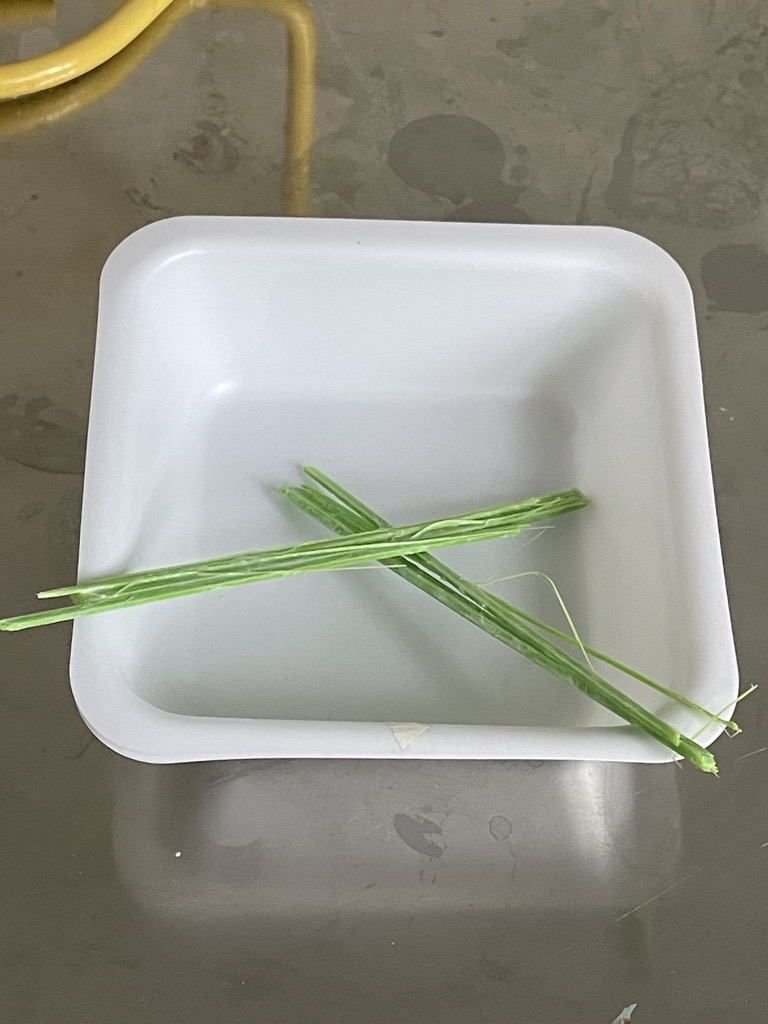
\includegraphics[width=1\linewidth]{Images/PLA_CUBIC_A.jpg}
    \caption{Severely damaged remains of PLA mount after clearing attempt}
    \end{subfigure}
    ~
    \begin{subfigure}[t]{0.4\textwidth}
    \centering
    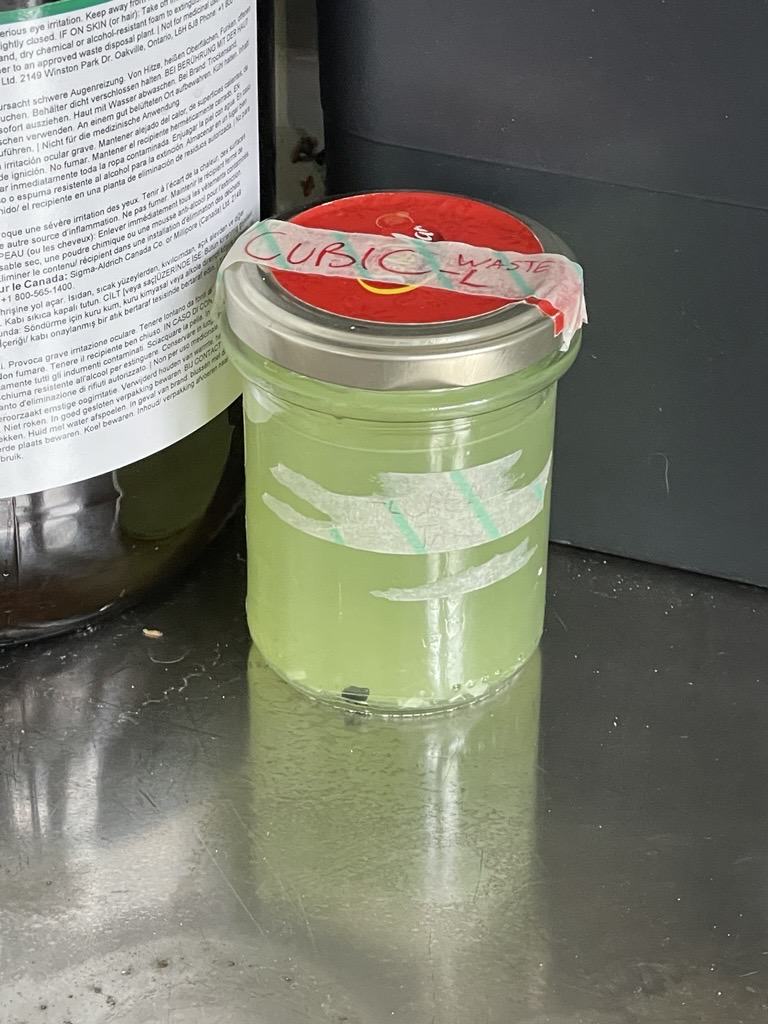
\includegraphics[width=1\linewidth]{Images/PLA_CUBIC_B.jpg}
    \caption{CUBIC-L solution saturated With PLA dye after clearing attempt}
    \end{subfigure}
    \medskip

\label{fig:enter-label}
\caption{\textbf{Degradation of 3D printed, PLA mount after exposure to CUBIC-L.} Mounted sample stored immersed in CUBIC-L for 21 Days at 37 degrees Celsius with gentle agitation.}
\end{figure}

Upon further research, it was determined that the N-butyldiethanolamine contained within the CUBIC-L was responsible for this result. The hydroxyl and amine groups of the chemical dissolved in the solution acted as a catalyst which accelerated the hydrolysis of the PLA, breaking down the material at the weakest points, splintering the material into the individual layers created by the 3D printing process []. This rate of degradation was likely only further accelerated by the high temperatures and stirring experienced by the mounts during the clearing time period. 

It was also observed in this test that a significant amount of dye from the PLA had also begun to leech into the clearing solution as the it had acquired a green hue in line with the original colour of the PLA material used by the test mounts (Figure 3.15(b)). This dissolved dye in the solution could cause a wide variety of complications to the clearing process should samples be exposed to it while immersed in CUBIC-L. Avoiding this outcome was seen as a top priority in any instance the mounts were used in the pipeline, thus all mounts fabricated after this test utilized natural coloured PLA containing no dyes for colouration as a precaution. It is recommended that dye free PLA be used for all mounts made for use at any point in the imaging pipeline. While no such dye contamination occurred when the mount is used in the CLARITY clearing and imaging, it is still a possibility worth avoiding altogether. 

\section{Chapter Summary}

This chapter detailed the pre-processing protocols implemented on all cardiac tissues examined throughout the course of this project. The discussion thereafter moved towards the subsequent tissue slicing performed on sliced tissue samples utilized followed by the two tissue clearing protocols utilized in this project: CLARITY and CUBIC-L/RA. To confirm clearing was completed properly and that the tissue structure had not been compromised by the clearing process, characterization experiments were performed for samples cleared using both techniques. Experimental results showed the tissue expansion, transparency, and structural preservation in samples cleared were found to be consistent with results seen in prior publications[,]. With the clearing protocols validated and tissue samples structure preserved for use in structural analysis post-clearing, the discussion turns to the means by which these samples are to be attached on the mesoSPIM microscope system. The design, installation, characterization, and data processing of the custom designed tissue mounting apparatuses is the focus of the next chapter and is the lynch pin by which the clearing and imaging steps of the imaging pipeline come together.



